%   Template for a LaTeX MSc Business Analytics Dissertation/Practicum
%   Sean McGarraghy and James McDermott
%   Remove these first three lines when starting your own document
%
%   MSc Business Analytics Dissertation/Practicum
%
%   Title:     Aaa Bbbbbbb Cccccccccc
%   Author(s): Xxxxxx Xxxxxxxxx and Yyy Yyyyyyyyy
%
%   This file is the top level file for a dissertation.  It contains:
%   - usepackage commands for any packages required
%   - document-wide parameter settings such as textwidth, etc
%   - The text of small items of the frontmatter (title, abstract, etc.) and backmatter
%
%   Chapter 1: Introduction and basic definitions
%   Chapter 2: Business background and problem
%   Chapter 3: Literature Review
%   Chapter 4: Methodology
%   Chapter 5: Results
%   Chapter 6: Discussion
%   Chapter 7: Conclusions
%
%   Change Control:
%   When     Who   Ver  What
%   -------  ----  ---  --------------------------------------------------------------
%   01Sep10  SMcG  0.0  Developed MSc Business Analytics Dissertation LaTeX template
%   02Sep16  JMcD  0.1  Updated template
%   01Apr17  XX    0.2  Begun dissertation proper
%   02Apr17  YY    0.3  Added ....
%

%% To LaTeX (compile) your whole document, run these 4 commands in the order given (I run them from
%% the command line on Linux or Mac OS X but you can run them from inside WinEdt or whatever you use):
%% latex  yourfilename
%% bibtex yourfilename  % NB this is the name of your LaTeX file, not your BibTeX database file!!
%% latex  yourfilename
%% latex  yourfilename
%%
%% Note: you don't need the .tex extension of yourfilename.tex (in fact giving it will confuse bibtex,
%% though latex will understand it).  If you stick with the name thesis.tex for this file, you would use
%% latex thesis etc
%%
%% There are two approaches to where to put the supporting files (LaTeX style (package) files, etc).  Either:
%% 1. Put them all in the same directory as this file (quick and dirty); or
%% 2. Many style (package) files such as natbib.sty, lineno.sty may already be installed on your system, but if
%%    not, just download them e.g., from ctan.org, and copy them to YOURBASEDIRECTORY/texmf/tex/latex
%%    Copy the BibTeX style file mscBA.bst to YOURBASEDIRECTORY/texmf/bibtex/bst
%% Approach 2 will make these files visible to any other LaTeX docs you produce.  Here, YOURBASEDIRECTORY is
%% typically your home directory.

\documentclass[a4paper,12pt,bibtotoc,notitlepage,oneside]{book}
% remove ``oneside'' when printing the final version since that
% will have plenty of blank pages already!

% the bibtotoc may be needed to make your references appear in the Contents, also liststotoc etc

% Preamble

% LaTeX Packages to use
\usepackage{makeidx}
%\usepackage{showidx} % for drafts: shows in margin what will be indexed
\usepackage{amsthm,amsmath,amsfonts,amssymb,latexsym,graphicx,appendix,subfigure}
% the ams* packages provide the (very useful) LaTeX extensions from the AMS (Amer. Math. Soc.)
% latexsym provides some useful extra symbols
% graphicx gives control over image files, e.g., width, etc
% appendix gives more fine-tuned control over the appendices
% subfigure lets you put multiple figures (and tables) in a figure environment, so you can refer to them individually, e.g., Figure~6(b).
\usepackage{algorithm2e} % handles algorithms in a nice way, akin to tables and figures
\usepackage[subfigure]{tocloft}  % package allows you to control the design of table of contents, figures and tables. use subfigure for compatibility -- jmmcd
\usepackage{natbib}   % gives more control over references and style of citation.  Has a lot of options, e.g., can use the [sectionbib] option to have multiple bibliographies in my document, listed in sections rather than chapters. Need this package for Chicago Manual of Style BibTeX referencing and the MScBA derived style
\usepackage{lineno}   % useful for early draft, so a reviewer can list by pageno+lineno where to make changes
% Packages you may like to use
% \usepackage{fancyhdr}  % more control over contents of page headers and footers for documentclass book
% \usepackage{psfrag}  % if using eps files for images, this package lets you replace text in those images, so you can have the same font type and size in both text and images.
% \usepackage{layout} % prints an overview of all the page margins, if you include \layout
%\usepackage[sectionbib]{natbib} if using multiple bibliography files
%\usepackage{chapterbib}
%\usepackage{doublespace} % for double spacing, e.g. initial versions for correcting
%\usepackage[nottoc]{tocbibind} % puts almost everything in the Table of Contents

% include your own macro / declaration files, if any
%   Macros
%   Esp. Theorem styles for amsart/amsbook document classes (currently enabled)
%
%   Sean McGarraghy
%
%   Change Control:
%   Date      Ver  Reason
%   --------  ---  --------------------------------------------------------------
%   12/05/98  0.1  Begun
%

\newcommand*{\Ax}  {Axiom~}
\newcommand*{\Df}  {Definition~}
\newcommand*{\Th}  {Theorem~}
\newcommand*{\Co}  {Corollary~}
\renewcommand*{\Pr}{Proposition~}
\newcommand*{\Lm}  {Lemma~}
\newcommand*{\Rk}  {Remark~}
\newcommand*{\Ex}  {Example~}
\newcommand*{\Exe} {Exercise~}
\newcommand*{\Eq}  {Equation~}
\newcommand*{\dfn} {definition}

\theoremstyle{plain}                 % Default

\newtheorem{thm}{Theorem}[chapter]
\newtheorem{lemma}[thm]{Lemma}
\newtheorem{lem}[thm]{Lemma}
\newtheorem{propn}[thm]{Proposition}
\newtheorem{pr}[thm]{Proposition}
\newtheorem{prp}[thm]{Propn.}
\newtheorem{cor}[thm]{Corollary}
\newtheorem{fact}[thm]{Fact}
\newtheorem{conj}[thm]{Conjecture}
\newtheorem{claim}{Claim}[]

\theoremstyle{definition}

\newtheorem{dm}{}  % Dummy theorem name for numbering only, independent of section
\newtheorem{dmy}[thm]{}  % Dummy theorem name for numbering only
\newtheorem{defn}[thm]{Definition}
\newtheorem{ex}[thm]{Example}
\newtheorem{exe}[thm]{Exercise}

\theoremstyle{remark}

\newtheorem{rmk}[thm]{Remark}
\newtheorem{notn}[thm]{Notation}
\newtheorem{note}[thm]{Note}
\newtheorem{cmt}[thm]{Comment}
\newtheorem{case}[thm]{Case}
\newtheorem{intr1}[thm]{Introduction}
\newtheorem{intro}[thm]{Introduction}

\newenvironment{pf}{\vspace{-4pt}\noindent\begin{proof}}{\end{proof}\vspace{2pt}}




%   General LaTeX Declarations (try -adobe-courier-medium-r-normal--18-180-75-75-m-110-iso8859-2)
%
%   Sean McGarraghy
%
%   Change Control:
%   Date      Ver  Reason
%   --------  ---  --------------------------------------------------------------
%   12/02/98  0.1  Begun
%

% Where to hyphenate words LaTeX doesn't know

\hyphenation{neigh-bour-hood neigh-bour-hoods}
\hyphenation{Bel-field}

% Short commands for italic, bold etc fonts

\newcommand*{\tr}[1]{\textrm{#1}}
\newcommand*{\ti}[1]{\textit{#1}}
\newcommand*{\tb}[1]{\textbf{#1}}
\newcommand*{\ts}[1]{\textsl{#1}}
\newcommand*{\tc}[1]{\textsc{#1}}
\newcommand*{\mr}[1]{\mathrm{#1}}
\newcommand*{\mb}[1]{\mathbf{#1}}
\newcommand*{\tth}[1]{{\slshape #1}}
\newcommand*{\df}[1]{\textbf{#1}}      % put the thing being defined in bold

\newcommand*{\bs}{$\backslash$}
\newcommand*{\ol}[1]{\overline{#1}}
\newcommand*{\cnj}[1]{\overline{#1}}
\newcommand*{\nth}[1]{\ensuremath{{#1}^{\textrm{th}}}}% superscripted `th' for counting
\newcommand*{\nst}[1]{\ensuremath{{#1}^{\textrm{st}}}}% superscripted `st' for counting
\newcommand*{\nnd}[1]{\ensuremath{{#1}^{\textrm{nd}}}}% superscripted `nd' for counting
\newcommand*{\nrd}[1]{\ensuremath{{#1}^{\textrm{rd}}}}% superscripted `rd' for counting

% commonly occurring text in Maths documents

\newcommand*{\eg}  {e.\,g.~}
\newcommand*{\ie}  {i.\,e.~}
\newcommand*{\ff}  {\textrm{if and only if }}
\newcommand*{\A}   {\textrm{ for all }}
\newcommand*{\all} {\textrm{ for all }}
\renewcommand*{\AA}{\ensuremath{\forall~}}
\newcommand*{\E}   {\textrm{ there exists }}
\newcommand*{\EE}  {\ensuremath{\exists~}}
\newcommand*{\st}  {\textrm{ such that }}
\newcommand*{\sta} {\textrm{ such that, for all }}
\newcommand*{\tfae}{the following are equivalent}
\newcommand*{\Tfae}{The following are equivalent}
\newcommand*{\wrt} {with respect to }
\newcommand*{\wolog}{without loss of generality}
\newcommand*{\Wolog}{Without loss of generality}
\newcommand*{\ftsoc}{for the sake of contradiction}
\newcommand*{\resp}{respectively}
\newcommand*{\RHS} {right hand side}
\newcommand*{\LHS} {left hand side}
\newcommand*{\Pf}  {\noindent\tb{Proof: }}            % for backwards compatibility only
\newcommand*{\eop} {~~\vrule height 5 pt width 5 pt depth 0 pt\relax}
\newcommand*{\QED} {\mbox{}\hspace{\fill}\eop}

\newcommand*{\fn}  {function}
\newcommand*{\vsp} {vector space}

\newcommand*{\ind} {independent}
\newcommand*{\dep} {dependent}
\newcommand*{\lcmb}{linear combination}
\newcommand*{\lind}{linearly independent}
\newcommand*{\ldep}{linearly dependent}
\newcommand*{\di}  {dimension}
\newcommand*{\fd}  {finite-dimension}
\newcommand*{\cp}  {characteristic polynomial}
\newcommand*{\de}  {determinant}
\newcommand*{\evl} {eigenvalue}
\newcommand*{\evc} {eigenvector}
\newcommand*{\sle} {system of linear equations}
\newcommand*{\ERO} {elementary row operation}
\newcommand*{\ECO} {elementary column operation}
\newcommand*{\repn}{representation}

\newcommand*{\UCD} {University College Dublin} 

\newcommand*{\itema}[1][a]{\item[(\emph{#1})]} 
\newcommand*{\ita}[1][a]{(\emph{#1})} 

% Math Roman abbreviations e.g. Gal(), Aut() etc.

\newcommand*{\len}{\ensuremath{\operatorname{length}}}% 
\newcommand*{\rank}{\ensuremath{\operatorname{rank}}} % RANK of matrix/linear map
\newcommand*{\nll}{\ensuremath{\operatorname{nullity}}} % NULLity of linear map
\newcommand*{\diag}{\ensuremath{\operatorname{diag}}} % DIAGonal matrix
\newcommand*{\cond}{\ensuremath{\operatorname{cond}}} % CONDition number
\newcommand*{\sign}{\ensuremath{\operatorname{sign}}} % SIGNature
\newcommand*{\sgn} {\ensuremath{\operatorname{sgn}}}  % SiGN of permutation
\newcommand*{\imp}{\ensuremath{\mathbin\Rightarrow}}  % IMPlies sign
\renewcommand*{\Im}{\ensuremath{\operatorname{Im}}}   % IMage (of a map)
\newcommand*{\zv} {\ensuremath{\mathbf{0}}}           % Zero vector
\newcommand*{\zs}[1]{\ensuremath{{#1}^{-1}(0)}}       % Zero Set of function #1
\renewcommand*{\i}[1]{\ensuremath{{#1}^{-1}}}         % Inverse of geezer #1

% spacing/heading commands

\newcommand*{\cpb}{\vspace{\fill}\pagebreak}          % Clean PageBreak inside paragraph
\newcommand*{\cb}{\hspace*{\fill}\\*[\medskipamount]} % Clean Break inside paragraph
\newcommand*{\cbb}{\hspace*{\fill}\\[\medskipamount]} % Clean Break, may have page Break
\newcommand*{\cbs}{\hspace*{\fill}\\*[\smallskipamount]} % Small Clean Creak inside paragraph
\newcommand*{\cbbs}{\hspace*{\fill}\\[\smallskipamount]} % Small Clean Creak, may have page break
\newcommand*{\cbl}{\hspace*{\fill}\\*}                % No gap Clean Break inside paragraph
\newcommand*{\cbbl}{\hspace*{\fill}\\}                % No gap Clean Break, may have page break

\newcommand*{\qt}[1]{\ensuremath{\quad\text{#1}\quad}}
\newcommand*{\qqt}[1]{\ensuremath{\qquad\text{#1}\qquad}}

\newcommand*{\subhead}[1]{  
            \begin{center}
            \tb{#1}
            \end{center}\\*}


% Various inclusion, ideal, equivalence, mapping symbols

%\newcommand*{\squig}{\sim\!\sim\!\rightarrow}  % old definition
\newcommand*{\eqv} {\ensuremath{\mathbin\Leftrightarrow}}  % EQuiValence sign
\newcommand*{\app} {\ensuremath{\rightarrow}}          % APProaches/tends to (limit)
\newcommand*{\map} {\ensuremath{\longrightarrow}}      % set MAPs to (long arrow)
\newcommand*{\tmap}[1]{\ensuremath{
                      \stackrel{\ssk{#1}}{\map} }}    % scriptsize #1 atop ---> arrow
\newcommand*{\mpt}{\ensuremath{\longmapsto}}          % element maps to (long arrow with bar)
\newcommand*{\tmpt}[1]{\ensuremath{
                               \stackrel{#1}{\mpt}}}  % scriptsize #1 atop |--> arrow
\newcommand*{\cng}{\ensuremath{\equiv}}               % CoNGruent to 
\newcommand*{\rel}{\ensuremath{\sim}}                 % single tilde RELation sign
\newcommand*{\nul}{\ensuremath{\emptyset}}            % NULl set 
\newcommand*{\su} {\ensuremath{\subset}}              % SUbset of
\newcommand*{\se} {\ensuremath{\subseteq}}            % Subset of/Equal to
\newcommand*{\sne}{\ensuremath{\subsetneqq}}          % Subset of but Not Equal to
\newcommand*{\sm} {\ensuremath{\smallsetminus}}       % set difference (Set Minus)
\newcommand*{\la} {\ensuremath{\langle}}              % Left Angle bracket
\newcommand*{\ra} {\ensuremath{\rangle}}              % Right Angle bracket
\newcommand*{\du} {\ensuremath{\dot{\cup}}}           % Disjoint Union (dot over cup sign)
\newcommand*{\rt}{\right}
\newcommand*{\lt}{\left}
\newcommand*{\oo}{\ensuremath{\infty}}                % oo = infinity
\newcommand*{\fp}[3]{\ensuremath{{#1}:{#2}\map{#3}}}  % Function/maP f:A--->B
\newcommand*{\ma}[3]{\ensuremath{{#1}:\R^{#2}\map\R^{#3}}} % MAp f:R^n--->R^m
\newcommand*{\lma}[4][]{linear map{#1} \ma{#2}{#3}{#4}} % linear map(s) f:R^n--->R^m
\newcommand*{\cpd}[1][A]{\ensuremath{\det({#1}-\l I)}} % char poly eg det(A-lI)

% Logic and proof
\newcommand*{\LT} {\texttt{T}}
\newcommand*{\LF} {\texttt{F}}
\newcommand*{\NOT}{\mathop\mathrm{not}}
\newcommand*{\AND}{\mathbin\mathrm{and}}
\newcommand*{\OR} {\mathbin\mathrm{or}}

% Binomial coefficient
\newcommand*{\bin}[2]{\ensuremath{\binom{#1}{#2}}}

% Binomial coefficient (textstyle i.e. Small font)
\newcommand*{\sbin}[2]{\ensuremath{\tbinom{#1}{#2}}}

% Binomial coefficient (displaystyle i.e. Big font)
\newcommand*{\bbin}[2]{\ensuremath{\dbinom{#1}{#2}}}

% derivatives
\newcommand*{\dd}[1]{\ensuremath{\displaystyle{\frac{d}{d{#1}}}}}

\newcommand*{\polyn}[3][n]{\ensuremath{{#3}_0+{#3}_1{#2}+\cdots+{#3}_{#1}{#2}^{#1}}}

% MATRICES

% two commonly used building blocks for matrices

% identity matrix
\newcommand*{\idmat}{\ensuremath{ 
1      & 0      & \cdots & 0       \\
0      & 1      & \cdots & 0       \\
\vdots & \vdots & \ddots & \vdots  \\
0      & 0      & \cdots & 1          } }

% matrix consisting of zeros
\newcommand*{\zeromat}{\ensuremath{ 
0      & 0      & \cdots & 0       \\
\vdots & \vdots & \ddots & \vdots  \\
0      & 0      & \cdots & 0          } }

% matrix consisting of asterisks
\newcommand*{\astmat}{\ensuremath{ 
*      & *      & \cdots & *       \\
\vdots & \vdots & \ddots & \vdots  \\
*      & *      & \cdots & *          } }

% Greek letters - abbreviations

\renewcommand*{\a}{\ensuremath{\alpha}}
\renewcommand*{\b}{\ensuremath{\beta}}
\newcommand*{\g}{\ensuremath{\gamma}}
\renewcommand*{\d}{\ensuremath{\delta}}
\newcommand*{\e}{\ensuremath{\varepsilon}}
\newcommand*{\z}{\ensuremath{\zeta}}
\newcommand*{\h}{\ensuremath{\eta}}
\renewcommand*{\th}{\ensuremath{\vartheta}}
%\newcommand*{\io}{\ensuremath{\iota}}
\renewcommand*{\k}{\ensuremath{\kappa}}
\renewcommand*{\l}{\ensuremath{\lambda}}
\newcommand*{\m}{\ensuremath{\mu}}
\newcommand*{\n}{\ensuremath{\nu}}
\renewcommand*{\r}{\ensuremath{\rho}}
\newcommand*{\s}{\ensuremath{\sigma}}
\renewcommand*{\t}{\ensuremath{\tau}}
\renewcommand*{\u}{\ensuremath{\upsilon}}
\newcommand*{\f}{\ensuremath{\varphi}}
\renewcommand*{\c}{\ensuremath{\chi}}
\newcommand*{\x}{\ensuremath{\xi}}
\newcommand*{\p}{\ensuremath{\psi}}
\renewcommand*{\o}{\ensuremath{\omega}}

\newcommand*{\G}{\ensuremath{\Gamma}}
\newcommand*{\D}{\ensuremath{\Delta}}
\newcommand*{\T}{\ensuremath{\Vartheta}}
\renewcommand*{\L}{\ensuremath{\Lambda}}
\renewcommand*{\L}{\ensuremath{{\textstyle{\bigwedge}}}}
%\newcommand*{\Si}{\ensuremath{\Sigma}}
\newcommand*{\U}{\ensuremath{\Upsilon}}
\newcommand*{\F}{\ensuremath{\Phi}}
\renewcommand*{\P}{\ensuremath{\Psi}}
\renewcommand*{\O}{\ensuremath{\Omega}}


% Math mode blackboard and calligraphic (script) letters

\newcommand*{\N}{\ensuremath{\mathbb{N}}}
\newcommand*{\Z}{\ensuremath{\mathbb{Z}}}
\newcommand*{\Q}{\ensuremath{\mathbb{Q}}}
\newcommand*{\R}{\ensuremath{\mathbb{R}}}
\newcommand*{\C}{\ensuremath{\mathbb{C}}}
\renewcommand*{\H}{\ensuremath{\mathbb{H}}}
\newcommand*{\FF}{\ensuremath{\mathbb{F}}}

\newcommand*{\sA}{\ensuremath{\mathcal{A}}}
\newcommand*{\sB}{\ensuremath{\mathcal{B}}}
\newcommand*{\sC}{\ensuremath{\mathcal{C}}}
\newcommand*{\sD}{\ensuremath{\mathcal{D}}}
\newcommand*{\sE}{\ensuremath{\mathcal{E}}}
\newcommand*{\sF}{\ensuremath{\mathcal{F}}}
\newcommand*{\sG}{\ensuremath{\mathcal{G}}}
\newcommand*{\sH}{\ensuremath{\mathcal{H}}}
\newcommand*{\sI}{\ensuremath{\mathcal{I}}}
\newcommand*{\sJ}{\ensuremath{\mathcal{J}}}
\newcommand*{\sK}{\ensuremath{\mathcal{K}}}
\newcommand*{\sL}{\ensuremath{\mathcal{L}}}
\newcommand*{\sM}{\ensuremath{\mathcal{M}}}
\newcommand*{\sN}{\ensuremath{\mathcal{N}}}
\newcommand*{\sO}{\ensuremath{\mathcal{O}}}
\newcommand*{\sP}{\ensuremath{\mathcal{P}}}
\newcommand*{\sQ}{\ensuremath{\mathcal{Q}}}
\newcommand*{\sR}{\ensuremath{\mathcal{R}}}
\newcommand*{\sS}{\ensuremath{\mathcal{S}}}
\newcommand*{\sT}{\ensuremath{\mathcal{T}}}
\newcommand*{\sU}{\ensuremath{\mathcal{U}}}
\newcommand*{\sV}{\ensuremath{\mathcal{V}}}
\newcommand*{\sW}{\ensuremath{\mathcal{W}}}
\newcommand*{\sX}{\ensuremath{\mathcal{X}}}
\newcommand*{\sY}{\ensuremath{\mathcal{Y}}}
\newcommand*{\sZ}{\ensuremath{\mathcal{Z}}}


\linespread{1.25}         % spacing between lines
\parindent0pt             % no paragraph indentation
\parskip\smallskipamount  % small space between paragraphs

%\setlength{ \topmargin      }{  -1cm }
%\setlength{ \textheight     }{  24cm }
\setlength{ \textwidth      }{  14cm }
\setlength{ \oddsidemargin  }{ 1.0cm }
\setlength{ \evensidemargin }{ 1.0cm }

\numberwithin{equation}{section}  % alter this if desired
\numberwithin{figure}{chapter}    % alter this if desired

\pagestyle{plain} % just puts a page number at the bottom of each page
% If you comment out the last line's \pagestyle command, you can control the page headers as follows:
%\def\leftmark{\textsc{YourText1}}  % text to appear in header of left-hand (even numbered) pages, e.g., Chapter Title
%\def\rightmark{\textsc{YourText2}}  % text to appear in header of right-hand (odd numbered) pages, e.g., Thesis Title
%\def\leftmark{\textsc{}}  % gives empty header on left-hand (even numbered) pages
%\def\rightmark{\textsc{}}  % gives empty header on right-hand (odd numbered) pages

% If, in the output, if you find the width of numbers in the Contents, List of Figures, etc is too great
% (e.g. too close to the heading names) uncomment the following
%\setlength{\cftfignumwidth}{3em} % this allows you to control width of numbering in List of Figures
                                 % 4em, 5em etc would be even wider; you can also hardcode 2cm or similar
                                 % but units of em (width of a capital M) or ex (height of a small x) are
                                 % preferred since they vary with the font type / size used

% comment this out for your final version (where you don't want line numbers)
%\linenumbers

\makeindex % generates the index entries (unsorted: need to run makeindex from the command line to sort them)


% Use the following to only include certain chapters (it will speed up compilation of the part you
% are currently working on, should the dissertation as a whole take excessively long to compile).
\includeonly{%
preface%
,
ch1%
,%
ch2%
,%
ch3
,%
ch4%
,
ch5%
,
ch6%
,
ch7%
,
appendix1%
,
appendix2%
,
glossary%
,
notation
}


%% Lay out your thesis as follows (standard book form: some of these are optional):

%% \begin{enumerate}
%% \item Front matter (preliminaries: roman page numbering, i, ii, iii, iv,\ldots)
%%   \begin{enumerate}
%%   \itema{} Title Page, giving (on separate lines, in this order):
%%     \begin{enumerate}
%%     \itema[i] Title
%%     \itema[ii] Author(s), listing previous degree(s), e.g.,\ Joe Bloggs, B.E.
%%     \itema[iii] A thesis submitted to \UCD\ in part fulfilment of the requirements of the degree of
%%           M.Sc.~in Business Analytics
%%     \itema[iv] Michael Smurfit Graduate School of Business
%%     \itema[v] Date (\emph{Month, Year}, e.g.,\ \emph{September, 2010})
%%     \itema[vi] Supervisor(s): Xxx Xxxxx (and Yyy Yyyyy)
%%     \itema[vii] Head of School: Professor Ciar\'an O'h\'Ogartaigh
%%  \end{enumerate}
%%   \itema[b] Dedication
%%   \itema[c] Table of Contents
%%   \itema[d] List of Figures (Illustrations)
%%   \itema[e] List of Tables
%%   \itema[f] List of Algorithms (if any)
%%   \itema[g] Foreword (if any: may precede table of contents)
%%   \itema[h] Preface (including authors' signatures: may precede table of contents)
%%   \itema[j] Acknowledgements (including permissions and other credits)
%%   \itema[k] Abstract
%%   \itema[l] List of important abbreviations (including special fonts, e.g.,\ {\tt fixed width} for program code)
%%  \end{enumerate}
%% \item Body or ``Main Matter'' (the text: arabic page numbering, 1, 2, 3,\ldots)
%%   \begin{enumerate}
%%   \itema{} Chapters of your dissertation, including, but not limited to:
%%     \begin{enumerate}
%% \itema[i] Introduction
%% \itema[ii] Literature Review
%% \itema[iii] Methodology
%% \itema[iv] Results
%% \itema[v] Analysis/Discussion
%% \itema[vi] Conclusions
%%    \end{enumerate}
%%   \itema[b] Epilogue (if any)
%%   \itema[c] Afterword (if any)
%%   \end{enumerate}
%% \item Back matter (loose ends: continue arabic page numbering)
%%   \begin{enumerate}
%%   \itema{} Appendices (if any: may include program code if not too long)
%%   \itema[b] Endnotes
%%   \itema[c] Glossary of terms
%%   \itema[d] Bibliography (References)
%%   \itema[e] List of contributors
%%   \itema[f] Notation Index / List of Symbols
%%   \itema[g] Index
%% \end{enumerate}
%% \end{enumerate}


\begin{document}

\frontmatter % This is the material before chapter 1, page numbering in Roman numerals ii, iii, iv, ...

\title%[Abbreviated Title for Header]
    {\bf Title of Dissertation/Practicum:\\
    An investigation of XYZ using ABC}

\author{Xxxxxx Xxxxxxxxx, B.E., and Yyy Yyyyyyyyy, B.Comm.}  % change to suit!
\date{}
\maketitle % this outputs the title using the \title and \author above

{\normalsize
\vfill
\begin{center}
% Alternative for PhD
%\textup{A thesis submitted to University College Dublin in part fulfilment
%of the requirements of the degree of Philosophi\ae~Doctor}
\textup{A Dissertation/Practicum submitted to University College Dublin in part fulfilment
of the requirements of the degree of M.Sc.~in Business Analytics}
\end{center}
\vfill
\begin{center}
Michael Smurfit Graduate School of Business,
University College Dublin
\end{center}
\vfill
\begin{center}
\textit{September, 2017}
\end{center}
\vfill
\begin{center}
\textup{Supervisors: Dr. Conor Reid and Prof. Yyy Yyyyy}
\end{center}
\vfill
\begin{center}
\textup{Head of School: Professor Ciar\'an \'O h\'Ogartaigh}
\end{center}
\vfill
}

\thispagestyle{empty} % it is conventional to have no page number on the title page (page i)

\clearpage % inserts a page break


% Subsequent distinct parts of the document begin with a \chapter*{} command: this produces a chapter with
% no number.  Note that in a book or amsbook document class, each chapter starts on a new odd-numbered page.


%% Dedication
\chapter*{Dedication}
To X, Y and Z (typically family members)


%% Table of Contents
% If you would like the word ``Chapter '' to appear before the chapter number in your Contents, uncomment:
% \renewcommand{\cftchapfont}{Chapter }

\cleardoublepage
\tableofcontents
%\renewcommand{\cftchapfont}{}

% Note: to show subfigures, subtables (if any) in the appropriate list below, uncomment the following command
% \setcounter{lofdepth}{2}

% If you find your Table and/or Figure captions are taking up too much space in the Lists below, use the
% following in the appropriate Table and Figure environments in your chapters:
%\caption[Short Caption]{An Excessively Long and Descriptive Caption, which is probably too long in any case\ldots}
% Then the short caption appears in the list, while the long one appears in the text under your Table/Figure.

% below, the \addcontentsline{toc}{section}{List of figures} etc ensures these lists appear in the contents

% similarly to the \renewcommand{\cftchapfont}{Chapter } above, you can have the words Table or Figure appear
% in front of every entry in the appropriate list by uncommenting as approapriate:
%\renewcommand{\cftfigfont}{Figure }
%\renewcommand{\cfttabfont}{Table }

\clearpage

%% List of Figures (Illustrations)
\listoffigures\addcontentsline{toc}{chapter}{List of figures}

\clearpage
%% List of Tables
\listoftables\addcontentsline{toc}{chapter}{List of tables}

%% List of Algorithms (if any): need to \usepackage{algorithm2e} for nice algorithm layout and this command
\listofalgorithms\addcontentsline{toc}{chapter}{List of algorithms}

%% modify titles with
%% \renewcommand{\cftXtitlefont}{\Huge\itshape}
%% Replace the X with either “toc”, “lof” or “lot” and use any font size you like.
%% Available font sizes are: \tiny, \scriptsize, \footnotesize, \small, \normalsize, \large,
%% \Large, \LARGE, \huge and \Huge.



%% foreword (if any: may precede table of contents)
\chapter*{Foreword}



%% Preface (including authors' signatures: may precede table of contents)
%   MSc Business Analytics Dissertation
%
%   Title:     Aaa Bbbbbbb Cccccccccc
%   Author(s): Xxxxxx Xxxxxxxxx and Yyy Yyyyyyyyy
%
%   Preface
%
%   Change Control:
%   When     Who   Ver  What
%   -------  ----  ---  --------------------------------------------------------------
%   11Feb11  AB    0.1  Begun
%

\chapter*{Preface}

% Some people like to put in a little quote (Knuth in particular loves this)

\begin{quote}
\noindent\textit{Men occasionally stumble over the truth, but most of them pick themselves up and
hurry off as if nothing had happened.}

\hspace{2cm}--- Winston Churchill
\end{quote}

Much of the front matter is optional. In particular, include things like a Dedication, List of Figures, List of Tables, List of Algorithms, only if there are enough of them to justify it and it would help the reader.

Don't include both a Foreword and a Preface since they perform similar roles.

The same goes for appendices, index, glossary, list of notation and terms at the end. Include if they would help the reader.

But always, of course, include the Bibliography.

\vspace{2em}

University College Dublin \hfill Conor Reid \\
\today 


%% Acknowledgements (including permissions and other credits).  Modify as appropriate

\chapter*{Acknowledgements}



%% Abstract

%\begin{abstract}
\chapter*{Abstract/Executive Summary}

%%   List of important abbreviations (including special fonts, e.g.,\ {\tt fixed width} for program code)

% Bulk of thesis. line numbers in arabic numerals, 1, 2, 3, ...
\mainmatter

\linespread{1.3} % adjust line spacing (if desired)

% \include all your chapters.  This automatically puts the material on a new page.  Recall that \chapter{} and
% \chapter*{} start a new chapter on a new odd-numbered page, but won't put extra empty pages along with \include
%   MSc Business Analytics Dissertation
%
%   Title:     Aaa Bbbbbbb Cccccccccc
%   Author(s): Xxxxxx Xxxxxxxxx and Yyy Yyyyyyyyy
%
%   Chapter 1: Introduction and basic definitions
%
%   Change Control:
%   When     Who   Ver  What
%   -------  ----  ---  --------------------------------------------------------------
%   11Feb11  AB    0.1  Begun
%
\chapter{Introduction}\label{C.intro}
{This chapter forms the introduction to the current study, laying out its motivations and aims. We begin with a background of the domain, followed by the business motivation for this study. We follow this with a summary of the academic contribution, the research goals and scope and end with an outline of the document structure as a whole.  }
\section{Background}
{This study is primarily concerned with the relationship between corporate governance and company performance, particularly with how the former can be optimised to positively influence the latter. Corporate governance is a widely discussed, debated and researched topic that is as relevant today as it has ever been. The governance of a company dictates it's policies and motivations, ensuring that all stakeholders \footnote{A stakeholder is someone who has a stake, or a personal interest, in the company. Employees, the local community and the media are all stakeholders.} have input to how the company is run and share a vision of where it is going. Governance policy also acts to mitigate financial and ethical pitfalls, by setting clear standards. Thus it is fair to say that corporate governance has a wide ranging influence within and also outside the company.\\\\
We frequently see instances of corporate governance failure, which can lead to disastrous consequences financially and reputationally. Reputation is often of high importance in both the public and private sectors, which can lead to a promotion of more ethical and fair behaviour in order to protect it. Instances where companies fail in this regard often make eye-catching  headlines, for example \cite{cnnUnitedAirlines}, \cite{telegraphVolkswagon} and \cite{kirkpatrick2009corporate}. In a hyperconnected world where news spreads quickly, the importance of a functioning governance structure is more important than ever. \\\\
The interests of different parties can conflict in any business, between entities such as the shareholders \footnote{A shareholder is often an investor who has equity in the company. They often have no personal interest in the company, solely financial.} or directors. There is much debate on how best to align these interests, with suggested initiatives like structuring executive compensation to be at least partly dependant on firm performance. Shareholder interests can also conflict with the interests of the wider public as a whole, or the stakeholders. This is especially true for companies that heavy rely on natural resources as a driver for business. In this case, sustainability not just of the company but of finite natural resources that the public depend on must be closely governed and managed. This is often the responsibility not just of those within the company, but those outside it too.  \\\\
It is reasonable to argue that corporate governance influences all aspects of the company, not least its economic success. \cite{moldovan2015learning} studied this relationship, collecting data on corporate governance and using it to predict corporate success as measured in various ways. They were able to learn models that did this successfully, resulting in a number of rules dictating governance of high performing companies. The current study uses this as a starting point, and looks to address some limitations within in a number of areas, outlined in section \ref{RGAS}. Modern work around causation is also studied, with a view to applying it in this domain. This would act to strengthen previously derived relationships, and presents an opportunity to study the deeper causal influencers of corporate economic success.}
\section{Business Motivation}
{\cite{moldovan2015learning} state the conclusions they reached in their research, and point to the business significance of each. For example, they found that for US based companies the number of women on the board of directors was positively connected to company performance. They also found that in Western Europe, companies should employ larger audit teams that in turn lowers the risk of bankruptcy. In Eastern Europe, their main finding is that an independent chairman best influences economic success.\\\\ 
The business benefit of the above is obvious. By deriving a number of relationships between economic success and corporate governance, the authors first prove that a relationship does in fact exist in the first place. That is, high corporate governance performance is strongly linked with success. Secondly they are able to put forward recommendations for governance best practice and show what elements are most influential, with geographic context. A key element of management is identifying levers with which to effect outcomes in a positive way, which leads into the motivation for this research.\\\\
We look to first verify some of the above findings, but also look to find new influencers of economic success by expanding the research to include other predictors outside of governance features. This would in effect expand the array of tools available to corporations for effecting economic change. We also aim to strengthen these findings by seeking causal influencers, which would add a hierarchical element to the range of levers for change and direct efforts to spaces that are most likely to yield real success. }
\section{Academic Contribution}
{A key element of this study is the exploration of causal research and the application of these techniques in this domain. There is continual active research in this area, with interested parties offering new techniques and thought processes for making steps towards proving causation in a variety of domains. To our knowledge, causation research has not be applied in the area of corporate governance and its effect on outcomes, and thus would represent a novel endeavour that stands to contribute to the field in a meaningful way. \\\\ 
For example, the rules proposed by \cite{moldovan2015learning} are backed by strong correlations drawn from highly accurate statistical model. They make no steps towards estimating a cause and effect element to those relationships, or any other type of deeper analysis. We propose that a significant academic contribution would be had by exploring how causality is reached and applying it here, to see if more can be said of the aforementioned rules. \\\\
As mentioned above, this study plans to expand the work of \cite{moldovan2015learning} to include other types of company actions and activity. This would help gain a more wholistic view of how economic success can be promoted across all company functions. }
\section{Research Goals and Scope}{\label{RGAS}}
{There are a number of key goals that this study aims to achieve. They are presented below, along with a discussion of how success will be measured at each stage.
\begin{enumerate}
\item{\bf {Reproduce the findings of \cite{moldovan2015learning}}.}\\
{As mentioned, \cite{moldovan2015learning} made findings that point to interesting relationships between corporate governance and company performance. It would be useful to use similar data to reproduce some of these findings using the same techniques as the authors.}
\item{\bf {Improve on these findings}}\\
Next, the aim is to improve on these results using three methods. The first involves considering other predictors of corporate success beyond governance, such as a company's social responsibility performance or their environmental impact. The second involves using alternative measures of corporate success itself, that may better reflect how successful a company is. These may take the form of more informative financial ratios etc. The third method involves using alternative statistical techniques with a view to improving model performance using the standard measures of model accuracy. There are a plethora of techniques and algorithms not considered in the original study that may prove useful. The way in which data is preprocessed may also be altered as part of this step. For example, the authors discretised corporate success and perform classification on the resulting data. It may be advantageous to perform regression analysis here to gain greater granularity.
\item{\bf {Apply modern work on causality.}}\\
{A number of conclusions on the influence of corporate governance on company performance have been reached, using established statistical analysis and subsequently discovered correlation. In order to strengthen these findings and and gain deeper insight into the underlying mechanisms of the domain, modern work in causality will be applied. This will involve significant research into the ways in which this can be achieved, including data requirements and required pre-processing. The aim here is to gain a much deeper understanding of the casual influencers of corporate economic success, to drive best practice and contribute to knowledge base in this area. }
\end{enumerate}
{It is equally important to discuss what is out of the scope of this study. A distinction is not made in this study between public and private companies, although regulations dictating how public companies must govern are often more stringent and strictly enforced than private companies. Regulations include preventative measures for avoiding bankruptcy etc. Privately held firms often how more freedom and flexibility here. This can be especially true when dealing with audits and so on. \\\\
Further, regulatory differences from country to country are not considered. Some countries may introduce certain taxation and laws that influence the decisions made by local companies, like a carbon emissions tax that may make companies take their environmental footprint more seriously.} 
}
\section{Document Outline}
{This report is laid out as follows. Chapter \ref{C.LitReview} contains a brief literature review of this topic including how corporate success can be measured, other predictive corporate features that may be included, a review of other similar studies and concludes with a summary of research in the area of causation. Chapter \ref{C.Methodology} contains details of this studies methodology, including a summary of the data used and its pre-processing, algorithms used and methodology around applying casual techniques. Chapter \ref{C.Results} contains the results of this study. Included in chapter \ref{C.Discussion} is a discussion of these results, with some concluding remarks and opportunities for future research outlined in chapter \ref{C.Conclusions.Future.research}.      }

%   MSc Business Analytics Dissertation
%
%   Title:     Literature Review
%   Author: Conor Reid
%
%   Chapter 3: Literature Review
%
\chapter{Literature Review}\label{C.LitReview}
\section{Introduction}\label{S.intro3}
{It is natural in business to seek to optimise all aspects of corporate activity, with a view to positively effecting the bottom line. This is reflected in the literature on this domain, which considers the problem in a number of different forms, following a wide range of methodologies and researching often quite different results. We review a snapshot of this literature here. \\\\
We first present some of the ways that corporate success can be quantified. We look at how it is defined by \cite{moldovan2015learning}, as well as by others whose approaches may benefit this study. Also included here is a discussion of various fronts on which companies act, such as their corporate social responsibility commitments, with a view to including these aspects in this analysis as independent explanatory features. This is followed by an analysis of existing literature on the relationship between corporate governance and company performance, again including the work of \cite{moldovan2015learning} as well as other relevant studies. We then explore the literature regarding causation and the statistical techniques used to infer causation, with consideration of how these can be realised in this domain. There is also discussion on the issues that arise in attempting to do so, and how they can be addressed. This chapter finishes with a summary of the research gap that this study aims to address. }
\section{Company Performance - Measures and Influencers}\label{comPerform}
\subsection{Introduction}
{Among the key aspects of this study is the quantifying of corporate success, in a way that accurately represents {\it "good"} and {\it "bad"} corporate performance. There are many ways to do this, one of the most simple of which is to use financial ratios. Uncountable ratios have developed, each attempting to assign numerical performance ratings to companies and differing from one another by the accounting indictors considered and the aggregation of these indicators. \cite {eidleman1995z} outlines the patterns that ratios tend to follow. He states that these ratios are mostly created by academic researchers, who constantly derive new ways of combining individual metrics together to facilitate meaningful comparison between companies. First, researchers find a sample of companies that meet some predetermined criterion of failure, as well as another sample of comparable firms (size, industry etc) that differ only in financial health. A number of ratios are developed and tested against this dataset to determine which returns values that are consistently and significantly different for each group. Those which do so successfully are kept, the rest are discarded. Weights are assigned to each ratio to reach an aggregate equation. New firms are scored, and real-world performance recorded to measure how useful the new ratios are in practice. \\\\
This study primarily considers corporate governance features as predictors of corporate economic success. This follows the lead of \cite{moldovan2015learning} who do the same. Having said this, an aim of this study is to expand the range of predictors considered, and to this end we discuss alternative sources of company data that can be incorporated into the model. Perhaps the inclusion of more varied and diverse independent features, such as a companies social responsibility commitments or their impact on the environment can enhance overall understanding in this domain. These areas are discussed in this chapter.    }
\subsection{Financial Ratios}\label{FinancialRatios}
{Some financial ratios are more useful than others, varying significantly in complexity, in what particular aspects of a company they consider and also in how they combine those measures. This section includes a discussion of some of the most commonly used ratios, with comments on how best they can be used and in what context they are most powerful. \\\\
One of the indicators of corporate economic performance used by \cite{moldovan2015learning} is Tobin's Q score. This measure was devised by \cite{tobin1969general} who postulated that the combined market value of a given company should be equal to their replacement costs. When a companies replacement cost is equal to its market value, it is said to be in an ideal state. Any deviation either way, a ratio above or below 1, indicates future investment or the selling of assets respectively. \cite{moldovan2015learning} argue that the Q score allows the estimation of intangible assets, and is thus a worthy inclusion as a dependant measure of corporate success. Intangible assets drive market value up, rising the Q score.  \\\\
The use of this measure is well established in the literature, by \cite{chung1994simple}, 
\cite{bhagat2008corporate} and \cite{bolton2011unified}. \cite{chung1994simple} state that Tobin's Q plays an important part in financial interactions, and is employed to explain diverse corporate phenomena during the  decision making process for investment opportunities. \cite{bolton2011unified} used Tobin's Q to propose a model for dynamic investment and risk management and found that investment is best driven by an aggreagte model of which the Q score plays an important role. \\\\
The formal definition of Tobin's Q is presented by \cite{chung1994simple}, along side a much more simplified and conservative approximation of the authors making. This less complex definition is seen commonly in literature, for example by \cite{wahba2008does}. This formulation is given below as; \\
\begin {equation}\label{TobinQ}
(Approximate) \quad q  = \small {\frac{MVE + PS + DEBT}{TA}}
\end{equation}\\
Here, $MVE$ represents the product of a companies share price and count of common outstanding stock shares. $PS$ represents the liquidating value of the companies preferred stock. $DEBT$ represents the companies short-term liabilities minus its assets, also short-term. Finally, $TA$ represents the book value of the total assets of the company. In layman terms, assets that cannot be easily quantified can not always be entered in a companies books, but do always contribute to the share price of that company. Thus, a firm with lots of this type of asset will have a high Q score, and those without will have a low score.\\\\ 
There is debate as to the practically of the Q score. Intuitively, the Q score places a very high importance on one specific aspect of a business. For example, before WhatApp was acquired by Facebook it had very little concrete physical assets (i.e. those that could be recorded in their accounts). Rather, it had a platform with approximately 400million users, and a very high Q score. After purchase, the Q score would have dropped significantly since the amount Facebook paid would become the concrete asset recorded in their books. This is not to say that the Q score is a bad success indicator, but rather it may not fully represent the real value of a company at a given time.\\\\    \cite{chung1994simple} state in their research that the Q score is often neglected in real-world situations. One of the reasons they give for this is the complexity of the necessary calculations, and a potential unfamiliarity with its operational intricacies. Another reason is the unavailability of relevant data, particularly of sufficiently high accuracy and instantaneous availability. To counteract this, they worked to create and test an accurate approximation of Tobin's Q that utilises only basic financial information, show in equation \ref{TobinQ}.  They conclude that their approximation is close enough to the more formal definition to be used where more exhaustive calculations are not possible. \\\\
%\cite {dybvig2010tobin} criticise Tobin's Q more strongly, stating that it is fundamentally malformed as a measure of corporate performance. They highlight long-serving managers as risk adverse, and who "...can {\it enjoy the quiet life} and underinvest". A logical implication of this is that firms invest less and operate well below their profit-generating capacity and thus reduces their net-present value. However, such is Tobin's Q formulated, underinvestment by a firm increases its Q score. They go on to explain the scores ambiguity, COME BACK TO. \\\\
Another measure of corporate success used by \cite{moldovan2015learning} is the Altman Z score, which can be used as a probabilistic measure of whether a company will fall into bankruptcy within the next two years. It can also be used more generally as a financial distress measure and to predict corporate defaults. The authors point out that there is much advocacy in the literature for using this measure, and this study was unable to find any that strongly reject its usefulness. The Altman Z score is given as;
\begin {equation}\label{AltmanZScore}
\begin{aligned}
Z \ Score \quad = \quad & 1.2\bigg(\frac{Working \ Capital}{Total \ Assets}\bigg) \ + \\\\
		& 1.4\bigg({\frac{Retained \ Earnings}{Total \ Assets}}\bigg) \ + \\\\
		& 3.3\bigg({\frac{Earnings \ before \ Interest \ and \ Tax}{Total \ Assets}}\bigg) \ + \\\\
		& 0.6\bigg({\frac{Market \ Value \ of \ Equity}{Total \ Liabilities}}\bigg) \ + \\\\
		& 1.0\bigg({\frac{Sales}{Total \ Assets}}\bigg)
\end{aligned}
\end{equation}\\
Among those that support this scores use is \cite {eidleman1995z}, who discusses its use in practice. He begins by highlighting Altman's own tests using the Z score which involved predicting 72\% of bankruptcies two years prior to the event, although the sample size or companies involved are not mentioned. Eidleman argues that the Z score is tried and tested, and ``it has been demonstrated to be quite reliable in a variety of contexts and countries.'' \cite {eidleman1995z}. \\\\
Eidleman also outlines circumstances that warrant corrections and alterations to equation \ref{AltmanZScore}, in order to generalise it beyond its originally intended means. He argues that before being able to use the Z score, one must ensure the company in question is comparable to those involved in Altman's original study. Altman considered manufacturing and small firms in his original analysis, thus corrections must be made before scoring companies in different industries. Eidelman points to two specific circumstances here. \\\\
The first considers privately held companies, whose stocks are no publicly traded meaning term four of equation \ref{AltmanZScore} cannot be calculated. To correct for this, the Z score can be re-estimated using book values of equity. In other words, details from balance sheets published by private firms voluntarily can be used rather than details gleamed from the stock market. Certainly a work-around here is to consider solely publicly traded companies. A consequence of this is that such an analysis would only include companies that are bound by the the corporate governance code in their jurisdiction, which would need to be taken into account in studies such as this one.\\\\ Eidleman's second consideration is for non-manufacturing firms. The fifth term of equation \ref{AltmanZScore}, according to Eidleman, varies significantly by industry. He argues that merchandise firms for example, are significantly less capital intense and thus are much more likely to enjoy higher asset turnover and consequently Z-Scores. Z scores then would be likely to under-predict bankruptcy in these cases. In order to correct for this, a recommendation comes from Altman to eliminate the fifth term and adjust the weights. 
\clearpage
The adjusted equation \ref{AltmanZScoreAjusted} is shown below;
\begin {equation}\label{AltmanZScoreAjusted}
\begin{aligned}
Z \ Score \quad =  \quad & 6.56\bigg(\frac{Working \ Capital}{Total \ Assets}\bigg) \ + \\\\
		& 3.26\bigg({\frac{Retained \ Earnings}{Total \ Assets}}\bigg) \ + \\\\
		& 6.72\bigg({\frac{Earnings \ before \ Interest \ and \ Tax}{Total \ Assets}}\bigg) \ + \\\\
		& 1.05\bigg({\frac{Market \ Value \ of \ Equity}{Total \ Liabilities}}\bigg) \ \\\\ 
\end{aligned}
\end{equation}\\
Overall, the Altman Z score seems a highly appropriate indicator of corporate financial strength and thus success, and one that should be considered in this study. Consideration will need to be had for the type of industry included in this analysis, that will inform the exact calculation of the Z score itself. }
\subsection{Environmental Considerations}\label{EnvironmentalConsiderations}
{As mentioned previously, there is likely much room for improvement in the range of predictors of success considered in this analysis. One potentially useful area to consider is the environmental performance of the company, studied by \cite{schaltegger2002link}. The authors primary focus is on environmental management, specifically as a vehicle for corporate success. It is assumed here that environmental management and performance relate to the controlling of costs relating perhaps to the mining of natural resources. This may also refer to fines, penalties or taxes that are incurred due to harmful emissions, which must be carefully managed within a company to mitigate against. \\\\
The authors present two conflicting viewpoints in this space. The first states that improved environmental performance predominantly causes an increase in operating costs, due to investment and so on which in turn negatively effects the profitability of the company. The second viewpoint states the opposite; improving a firms environmental performance in fact induces cost savings, which drives increases in profitability. Interestingly, the authors present opinions that environmental investment often both negatively increases costs and positively increases income. Having said this, they argue that such a direct link is not present in practice, and that instead it is the identification and management of the relationship that is more important. The conflicting viewpoints are visualised in figure \ref{ch3_successAndEnviornment}. 
\begin{figure}[h] 
\centering
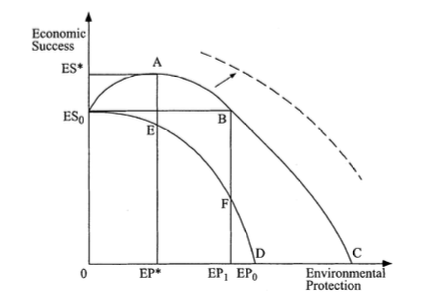
\includegraphics[scale = 0.7]{images/ch3_successAndEnviornment.png}
\caption{Correlation between corporate environmental protection spending and economic success (Source: \cite{schaltegger2002link}).}
\label{ch3_successAndEnviornment}
\end{figure}\\
$ES_0$ on the vertical axis represents the current level of economic success, described by the authors a certain shareholder value. According the the pessimistic view of environmental spending, this value decreases as spending in environmental protection increases (through points E and F, to D where non profit can be made). That is, spending in this space reduces profit making ability to eventual zero. The more optimistic view is represented by the path from $ES_0$ through points A and B to point C (again where no profit is possible). This represents the ideology that some economic gain can be achieved, at least to some degree before tailing off, by being environmentally conscious. Of course, even in this situation there is an optimal investment level, after which profit making ability decreases. \\\\
The authors draw point to two important ideas, derived from figure \ref{ch3_successAndEnviornment}. First, they argue that environmental performance can vary at a given level of economic success. It is both possible to be equally successful by being either environmental friendly or harmful. This indicates that investment in this space does not necessarily mean poor economic performance. Secondly, the reverse; that economic success can vary for a given level of environmental protection. That is, being environmentally conscious is no guarantee of economic benefit. The authors reiterate that the correlation between economic and environmental performance depends on not just company externalities but internal variables which are influenced by management. It is firm management, who moderate this relationship, that must be optimised in order to gain economically. The authors put this forward as an group of explanatory covariates not considered in the literature to this point. \\\\
It is natural then to ask how environmental management can be quantified in data for analysis. \cite{schaltegger2002link} suggest two cases for deriving data. The first relates to the firms ability to utilise to the full the economic benefits of environmental protection measures. This may materialise in R\&D spending, or other marketing positioning that communicates their efforts and establishes the company as industry leaders. They are seen as quality leaders, with their environmental management policies a significant driver of this. The second case relates to how this reputation is achieved in practice, by realising the optimal environmental performance for maximum economic success. This can take the form of identifying and implementing optimise production processes for example, facilitated by the identification of opportunities and "eco-efficiency potentials". \\\\
\cite{wahba2008does} also performs research in this area, studying whether the market values corporate environmental responsibility, specifically in an Egyptian context. Similarly to \cite{schaltegger2002link}, the author acknowledges divided and inconclusive literature on this topic, stating an aim to present empirical evidence on how engagement with environmental responsibility can positively influence corporate market value. This analysis looks at a sample of 156 firms across 19 industries, using the market value of a firm as the dependant variable (interestingly, quantified by Tobin's Q score mentioned previously). Important to note is the authors use of ISO 14000/14001 certification as a proxy for environmental performance. This is recognised by the authors as non-ideal, however this may still have some utility in future research to address the difficulty in quantifying performance in this area. \\\\
An interesting and important consideration is made by \cite{wahba2008does}. She states that companies with greater economic success have a greater ability to invest in environmental endeavours, leading to a theory that the two may be jointly determined. This theory is tested before regression analysis run. To do this, the author uses the specification test of \cite{hausman1978specification} to test for endogeneity. Endogeneity occurs in econometrics when an explanatory variable correlates with the error term, rather than some other feature. \cite{wahba2008does} states that the result of this analysis is that endogeneity is not occurring, but points to an important consideration that the current study may need to take into account. One of the common causes of this is a causal loop between an independent and a dependant variable, and can obviously lead to wildly inaccurate results. \\\\
 \cite{wahba2008does} state that the overall finding of this research is that the market does in fact reward firms for their environmental efforts, by positively influencing that firms Tobin's Q score, but do point to similar issues raised by \cite{schaltegger2002link}. Namely, that a companies decision to reduce their impact on the environment comes with significant cost and that if this is not managed correctly, the economic benefits evaporate.     \\\\
There is clear support in the literature for the presence of a relationship between corporate economic success and environmental performance. \cite{schaltegger2002link} suggest it is the firm management of environmental considerations that influences success, and put this forward as an explanatory variable not yet considered in literature. This theory is supported by \cite{wahba2008does}, who find a strong relationship in this space but with a caveat that management plays a significant role in realising benefits. It remains to be seen exactly how this can be realised in data analysis, and what family of covariates could be incorporated into the model.  }
\subsection{Corporate Social Responsibility}
{Corporate social responsibility, or CSR, is defined by the European Commission as "the responsibility of enterprises for their impacts on society". This is similar to being conscious of environmental impact, but is more generalised to include compliance with established ethical standards and national and international norms. Central to CSR is the creation of shared value between themselves, their stakeholders and larger society as well as mitigating possible adverse events with those groups. It is natural to consider elements of CSR then, when discussing predictors of firm success. \\\\
\cite{orlitzky2003corporate} perform meta-analysis in the link between corporate social and financial performance. They begin by stating;
``Most theorising on the relationship between corporate social / environmental performance (CSP) and corporate financial performance (CFP) assumes that the current evidence is too fractured or too variable to draw any generalisable conclusions \cite{orlitzky2003corporate}.''\\\\
Their research aims to show this claim is unfounded, and that it is indeed possible to derive insight in this space by providing a more rigorous methodology for drawing such conclusions. They argue that researchers have attempted to find causal relationships between CSP and CSR, but have failed in part due to a failure to see vital differences between theory and operational applications. They also state that an aim of their research is to aggregate knowledge in the area, and highlight important findings they believe to be overlooked. This type of meta-analysis have been proven to provide value by considering a number of disparate and conflicting results holistically, by reaching an aggregate conclusion.\\\\
They present a number of hypotheses about the influence of CSP. They first state that CSP and CFP are positively related, regardless of industry and the context of the given study relating the two. They base this on a number of studies, stating that CSP is a vital form of "good management theory" that boasts competitive advantage by addressing stakeholder concerns quickly and fairly.  Secondly, they hypothesise on the temporal nature of this relationship, and further that there is a bidirectional causality between CSR and CFP. That is, there is a circular and virtuous causal relationship that governs performance in each area. This is supported by the idea that prior success in CFP facilitates positive engagement in CSP, due to increased responsibility and freedom at the managerial level. This conclusion mirrors that seen in section \ref{EnvironmentalConsiderations}, where it was theorised that increased economic success drives better environmental performance.\\\\
The third hypothesis put forward by \cite{orlitzky2003corporate} involves the underlying logic behind the correlation between CSP and CFP. The first is that CSP boasts managerial competencies and organisational efficiency, by enabling shared knowledge of the firm's market as well as social and political environments. Secondly they suggest that CSP is a driving factor behind the firm's reputation, and thus elicits significant goodwill from stakeholders. \\\\
The fourth and final hypothesis put forward involves the methodology used by previous studies to draw conclusions from. The authors here suggest that the variance in results seen across studies can be explained by sampling or measurement error, for example. \\\\
In order to support these claims, \cite{orlitzky2003corporate} perform a meta-analysis involving 52 studies across both CSP and CFP, resulting in a total sample size of 33,878 observations on which they perform their analysis. This analysis involves a statistical aggregation technique to be applied, which calculates the cumulative correlations across studies, correcting for variable elements of those studies to reach one "true score correlation ($\rho$)". Using this technique, the authors were able to explain 24\% of the cross-study variance in relation to the observed r value, which they suggest is significant. That is, by controlling for sampling and measurement errors across multiple studies, they could reduce the variation in results by 25\%. They suggest that this, strengthened with other analysis, supports their collection of hypotheses.\\\\
The authors compare their results with others who performed similar research. Key to this comparison is a discussion regarding the linkage between CSP and CFP. That state that other researchers have traditionally been concerned with the "Halo effect". That is, that correlation found (that CSP influences CFP) are due to the experimental procedure or are spuriously perceived. The authors here dismiss this, stating that the only logical halo link would be in the reverse direction. That is, that a company who are high financially successful may be scored highly in CSP regardless of factual information in that regard. They go further, and state that even this hypothetical (but more logical) argument is debunked by their meta-analysis which shows a strong directional (or temporal) link between CSP and CFP. \\\\
As as with environmental performance, there is clear evidence that corporate social performance (or perhaps more commonly, responsibility) is a worthy addition to this study. Along side governance features and the aforementioned environmental performance features, there is evidence that CSP can enhance predictive power and understanding in this domain.    }
\section{Corporate Governance and Company Performance}
\subsection{Introduction}
{In this chapter, we explore research that directly attempts to answer similar questions as the current study. That is, other works that look at the relationship between corporate governance and company performance, and attempt to characterise that relationship. This includes the work of \cite{moldovan2015learning}, whose research forms the basis for the current study. An analysis is made of their methodology and conclusions, as well as a deeper analysis of what areas can be improved upon.}
\subsection{Existing research}
{\cite{moldovan2015learning} made an attempt to find relationships between how a company governs and its economic success, using data mining techniques. They derived a dataset from the Bloomberg financial system, containing 50 independent corporate governance features on areas such as board room structure and the  companies yearly tax and interest liabilities. They considered three stock indexes; S\&P 500 (a collection of 500 American companies), STOXX Europe 600 and STOXX Eastern Europe 300. They complimented this with two dependant, target variables measuring corporate success. Those measures are Tobin's Q and the Altman Z Score, the details of which are outlined in section \ref{comPerform}. Using the aforementioned governance variables, they learned statistical models to predict {\it "good"} and {\it "bad"} company performance.\\\\
Interestingly, \cite{moldovan2015learning} decided to discretise Tobin's Q into two classes, either {\it "good"} for high scores or {\it "bad"} for low scores. The threshold used here was the the median Q score of the entire dataset. They carry out similar preprocessing on the Altman Z score, creating three classes and allocating observations to each based on performance before using a classification algorithm for learning purposes. While the authors cite this methodology in previous literature, it may prove interesting to carry out regression on the real-valued scores as well. We believe this alternative methodology may yield positive results, that would perhaps be more granular and more appropriate for this data. \\\\
The formulation of the Altman Z score use by \cite{moldovan2015learning} is also an area for potential concern. As discussed in section \ref{FinancialRatios}, Altman presents an alternative formulation for non-manufacturing companies, that prevents the under estimation of bankruptcy likelihood associated with using the score for such companies. It remains to be seen what kind of companies are included in the analysis of \cite{moldovan2015learning}, although should a significant number fall outside of the manufacturing industry then perhaps the alternative formulation should be used in the current study.   \\\\
Using a number of different algorithms, \cite{moldovan2015learning} were able to predict with accuracy corporate outcomes using governance features. Interestingly, all algorithms performed equally well for American and European datasets, indicating a low level of model dependance here. Results from the Eastern European dataset were less consistent across algorithms, attributed to missing data on the governance side.\\\\
As mentioned previously, the authors here were able to present some simple rules based on their models for corporate governance best practice. For example, they conclude that there is a positive correlation between a female presence on the board of directors in American companies, thresholding on 20\% presence for the benefits to be detected. An independent lead director in the same dataset was shown to incur a higher risk of bankruptcy as measured by the Altman Z score. In Europe, the authors came to a similar conclusion, stating that the presence of an independent lead director or former CEO on the board of directors resulted in poorer Tobin Q scores. Interestingly and contrary to the case in America, the presence of women on the board was negatively linked to performance. Finally, in Eastern Europe \cite{moldovan2015learning} found that a smaller director age range was positively related with performance. Altman Z scores improve significantly with an independent chairman, or female CEO. \\\\
--------------------\\
{\color{red}
Papers left to review here
\begin{enumerate}
\item{\cite{bauer2008impact}}
\item{\cite{creamer2010learning}}
\item{\cite{chen2015does}}
\end{enumerate}}
--------------------
}
\section{Inferring Causation}
\subsection{Introduction}
{It is stated ad nauseum in scientific and popular literature that {\it "Correlation does not imply causation"} or similar. In statistical analysis, it is tempting to infer causal relationships between features where only correlation has been proven and indeed a significant amount of literature seems to do exactly this. For example, the study of \cite{moldovan2015learning} on which the current study is based, makes strong claims as to the relationship between corporate governance and company success. Here, the authors make a statement (among others) that Western European companies can expect to lower their Z-Score by employing a large audit committee, backed by an inverse relationship between the two. In reality, the authors perform insufficient analysis to support causal inference, instead finding correlations worthy of further investigation. \\\\
Interestingly, there is a significant body of research that argues that it is impossible to prove causation in any case. Logically, one must consider in their analysis all variables that could possibly prove to be casual, least a conclusion be drawn that leaves out some feature that in fact is the underlying casual factor for some observed phenomenon. Of course in practical studies this is almost never fully achieved due to real-world complexity, and so it may be that advanced techniques are required to move towards this case as much as possible to overcome this issue.  \\\\
One of the major issues with applying causality research in this domain is the study design. Many studies, particularly in the medical field, are able to take advantage of robust experimental design standards that facilitate a deep and accurate exploration of results. They are able to control for unobserved covariates using randomised trials, and generally have a large degree of control over the statistical parameters of the study. Study methodology here often follows a procedure of maintaining a treatment and control group. Researchers can then estimate the presence and magnitude of any observed relationship, and infer it to be caused by the treatment since that treatment is under the control of the researcher.  \\\\
Outside of such highly controlled experimental environments, causal inference becomes more difficult since we begin to deal with observational studies. The work of \cite{moldovan2015learning} is such a study, where the authors extracted historical data that was generated outside of their control and tried to uncover relationships within. \cite{esarey2015causal} identifies an interesting problem with this type of work. The author argues that often observations (whether they be people, organisations or events of some kind) self-select to be treated which has a significant effect on outcomes. He gives the example of education; those who choose to complete higher education may be those who stand to gain from it the most, and so it is difficult to estimate educations effect on income. If only those who really need education attend, then its positive influence on outcomes (a persons salary for example) would be skewed. Similarly in the study of \cite{moldovan2015learning}, it is difficult to assess the benefit of various elements of corporate governance on firm performance due to a possible self-selecting process undertaken by those who perform well in the former. \\\\
%There is an implicit temporal element to this discussion, and indeed \cite{pearl1995theory} state that often temporal precedence is normally assumed to be essential to defining a causal relationship. They argue that this alone cannot distinguish causation however, and point to research stating that unless one knows all potentially causal covariates it is impossible to make this step at all. \\\\
This is a highly complex space, and one that certainly calls for advanced techniques that can mitigate the issues outlined above. The remainder of this section is dedicated to some of these techniques, with discussion of their technicalities and practical applications.  }
\subsection{Matching}\label{matching}
{One approach to bridging the gap between experimental and non-experimental studies is matching, outlined by \cite{stuart2010matching} who considers studies that use observational data that can be divided into treated and non-treated cases. Matching is then used to study the effects of this treatment on some outcome, in a very similar way to standard experimental trials in the medical field for example. He describes first how one of the biggest benefits of randomised experimental studies is that the treated and un-treated groups are guaranteed to be randomly different from one another, on both observed and unobserved covariates (or features that may influence the outcome). That is, such experiments are able to control for factors that have not been explicitly designed for in the experiment. Statistical matching aims to imitate this for observational studies in which such design is very diffuclt, by balancing the distribution of potentially useful features in the treated and control groups. This is achieved by identifying observations that differ only in treated status, facilitating the analysis of the causal effect of that treatment. In effect this ignores un-observed features, and aims to reduce bias in the distribution of observed features as much as possible. The concept of {\it strong ignorability} is heavy relied upon here, which is to say that it is assumed that all feature that may influence the outcome are being considered. As mentioned previously, this is very difficult to achieve in practice. \\\\
\cite {stuart2010matching} states that matching is a potentially useful mechanism in supervised learning, where the outcome is known and the goal is to estimate its effect. Thus, matching is considered in this study where the treatment can be quantified as fluctuations in various explanatory corporate governance variables (among others) which in turn influence the a firms outcome. \\\\
\cite {stuart2010matching} sets out four key stages in the matching process. They are;
\begin {enumerate}
\item{Defining the measure of {\it closeness} between observations.}
\item{Choosing an appropriate matching method.}
\item{Quality assessment of matched samples, returning to step 1 depending on results.}
\item{Treatment analysis, given the results of Step 3.}
\end{enumerate}
A measure of closeness quantifiably determines whether an observation is a good match for another. This is a crucial aspect to matching, and can be subdivided into two parts. The first involves pruning the dataset features for those to include, taking into consideration the concept of {\it strong ignorability} mentioned earlier. \cite{stuart2010matching} points out that poor results are expected from using small sets of features, particularly those that pertain solely to a narrow view of that observation (for example, demographic details of individuals). He states that there is little disadvantage in including features that are not actually associated with outcome, albeit a slight increase in variance is expected. Conversely, neglecting a feature that is associated with outcome is very costly, and so it is recommended to include as many features as is practical as a precaution. In could be argued that this contradicts the authors earlier statements about ignorability, and so in this study some testing and iteration here is perhaps required. The authors also recommends to carry this out without relying on observed outcomes, and instead make decisions based on domain knowledge. This represents a trend in causal analysis, in that domain knowledge is heavily relied upon to strengthen correlation's rather than depending on deeper statistical analysis. \\\\
%put in something here about type of variables not to include
The second aspect to closeness is the measure of distance itself, or the similarity between two observations in the data. There are many ways to do this, that vary in the exactness of the match required. \cite{stuart2010matching} argues that exact matching is ideal, but very often unattainable especially with high dimensional data. Requiring a very high degree of exactness leads to observations remaining unmatched which then fall out of consideration, a phenomenon that in turn can lead to more bias than if the matching measure required less exactness. A way to address this is to categorise continuous features, a practice used in calculating the Mahalanobis distance for example which works well with low dimensionality, but poorly with highly non-uniformly distributed features.
\\\\ 
The next stage in the matching process is the choose of matching method, which uses the closeness distance to create the matches themselves. The motivation behind using one method over another lies in the number of observations that remain after matching has taken place, and the relative weights that different individuals receive. One such method is nearest neighbour matching (NNM), which is stated as the most common, most understandable and easiest to implement methods available by \cite{stuart2010matching}. In essence, this method couples a treated and un-treated observation, minimising the distance between the two. Controls can be put in place to dictate the exactness of each match, potentially discarding treated cases if a suitable match is not found. This helps to prevent bad matches, but leads to difficulties in interpreting results. What results from NNM is a data set of similar dimension to the amount of treated cases, which arguably reduces the power of the data. \cite{stuart2010matching} states in response to this that model precision is effected most by the smaller group size in any dataset, and so balancing observations down to this smaller group size should not in fact dramatically reduce it power. 
\\\\
The third stage of the matching process is a quality assessment of the matched samples, which is the most important step according to \cite{stuart2010matching}. The aim here is to rate how balanced the matches set is, where balance refers to the similarity of feature distributions, and the independence of features and treatment status. Poor results here calls for alternative distance measures and matching methods, and so iteration is often required to find the optimal methodology. \cite{stuart2010matching} proposes numerical diagnostics to achieve this step. This involves the inspection of the difference in means of each feature, divided by the standard deviation which gives the {\it standard bias}. This is performed for each feature, as well as their two-way interactions and squares. The author discards other common tests here such as hypothesis tests, due to contextual issues and how balance is interpreted by those tests. 
 \\\\ 
The fourth and final step of the matching process as outlined by \cite{stuart2010matching} is outcome analysis. It should be noted that matching is not actually a tool used for inferring causation, but rather presents a new dataset that is treated as if sourced through randomised methods.  
\\\\
\cite{king2014balance} also characterise the trade-off between matched sample sizes and the balance between classes into the matched subset, identified above by \cite{stuart2010matching}. While \cite{stuart2010matching} argued that any negative effects of sample reduction were offset by the increased balance between groups, \cite{king2014balance} argues the opposite. They claim that practitioners often do see sample reduction as an issue, citing manual tweaking that research cary out in an effort to optimise sample size as well as balance, or their tendency to settle for suboptimal solutions. \cite{king2014balance} argue that optimising only one of these parameters is not a viable solution nor a necessary one, but that current solutions available for optimising both require significant manual intervention which is time consuming and usually suboptimal. In response to this, they propose a new approach that they claim address a number of issues. \\\\
The so called {\it matching frontier} is a methodology that the authors claim fully characterises the trade-off between dataset imbalance and matched sample size, allowing researchers to visually inspect where the optimal solution lies for a given dataset. Each location along the frontier is denoted by the resultant matched sample. Moving along this frontier (i.e. varying sample size), the frontier returns a data subset such that no other subset of the same size has more optimal class balance characteristics. That is, the returned matched dataset is optimally balanced for its size. The implications of this for researchers are obvious. Using this method, one has much finer control over the matching process than is apparent in the work of  \cite{stuart2010matching}. The latter provides a framework that involves significant manual iteration, which is shown to be suboptimal and unnecessary by \cite{king2014balance}.\\
--------------------\\
{\color{red}
More to be said of work of \cite{king2014balance}\\}
--------------------}
\subsection{Minimal-Model Semantics}
{\cite{pearl1995theory} present a highly influential theory of causation, and guidelines on how to make the step from strong correlation towards inferring causal relationships. This is certainly one of the more influential studies in this space, and approaches the problem of causation slightly differently to matching laid out in section \ref{matching}. The authors here propose what they refer to as {\it a minimal-model semantics of causation}, which they claim debunks the myth that causal influences cannot be distinguished from illegitimate covariation. They argue such a distinction is possible by using inductive reasoning.\\\\
They begin by stating generalities of proving causation, and of causal systems. Firstly, they state that intelligent systems that aim to learn about their environment and act on that knowledge cannot rely solely on preprogrammed causal knowledge (derived from human knowledge and experience). Rather, it must be able to transform observable phenomenon into cause and effect relationships. This is a key point, and speaks to the statements of other authors who state domain knowledge is vital for causal inference. They argue further that when causal relationships are stated in ordinary conversation, they reflect probabilities of event occurring rather than absolutes. Thus, probability theory should be sufficient to identify such relationships. It is clear that the authors place a large degree of faith in the abilities of ordinary people, going as far as to say of peoples ability to perceive causal relationships; {\it "..we must find a computational model that emulates this perception"}.\\\\
Key to the model proposed by \cite{pearl1995theory} is the notion of a directed acyclic graph (DAG). The authors theorise that fundamentally, all processes in nature are controlled by causal mechanisms that govern how observable and unobservable variables interact. In general, they state that
``A causal model of a set of variables U is a directed acyclic graph (DAG), in which each node corresponds to a distinct element of U \cite {pearl1995theory}.'' \\\\
Variables are represented as nodes, with edges representing causal influences between those variables. Using this model, it becomes clear how the influence of parent variables on child variables can be found. One of the issues that has been raised in this chapter previously is that of the influence of unobservable factors, which are impossible to eliminate in observational studies in practice. The authors here model these factors as probabilistic disturbances to the DAG, that perturbs the relationships within. By stating assumption of independence of parent and child nodes (or features), the authors state that the disturbances are local to that pairing. This is certainly a novel approach, and presents a theoretical framework for dealing with inevitable externalities.\\\\
\cite {pearl1995theory} on go to discuss the question of model structure and choice. Logically, since the model $U$ is not bounded by any predetermined constraint (i.e. inputted causal knowledge or otherwise) there in an infinite amount of models that could be fitted to a given distribution. Each would create different causal relationships with a different set of probabilistic disturbances. The authors call on inductive reasoning here, arguing that any model can be removed if there is a more simple alternative that is as consistent with the data. Models not removed are referred to as {\it minimal models}, and are used to reach the authors definition of inferred causation. 
``A variable X is said to have a causal influence on a variable Y if a strictly directed path from X to Y exists in every minimal model consistent with the data  \cite {pearl1995theory}.''\\
{\color{red}
Much more to review in this paper including:
\begin{enumerate}
\item{More on the DAG structure - independence of parent / child}
\item{Stability - Computational Practicality}
\item{Latent Structures}
\item{Non-temporal causation}
\item{Attached algorithm to make this happen - see forked project at \url {https://github.com/ReidConor/causality}}
\end{enumerate}}
--------------------
\section{Research Gap}
{Over the course of this literature review we have present a snapshot of existing studies in this domain, and discuss their implications for the current research. It is clear that a large body of work exists in this space, that has promoted an ever deeper understanding of the drivers of economic success. Having said this, there are certainly gaps in this research left to be explored. In this chapter, we discuss the gaps that this study aims to address. \\\\
Firstly, it is clear that there is a wide range of plausible contributing factors to corporate economic success. We have seen evidence that governance, environmental investment and corporate social responsibility are all linked with success at least to some degree. However, we have not seen a study that collates these factors together in one study with a view to performing statistical analysis and deriving a much more diverse model. The literature contains numerous instances where the same measures of corporate success are relied upon, although there is questionable logic behind the decision to use them. Both of these points are addressed in this study; we attempt to consider as many potential predictors for success as is reasonable, as well as investigating measures of economic success that better represent what a successful or unsuccessful company is.\\\\
Perhaps the more significant gap that this research aims to address is that of the identification of causal relationships. Much work has gone into establishing correlative links between company behaviour and success, that are often reenforced with domain specific knowledge or simply accepted due to their plausibility by practitioners. The current research aims to negate the need for domain specific knowledge, by using cutting edge causal learning theory to pick out the correlations that in fact have causal elements to them. Such a study has not yet been carried out, and so the potential contribution to the field is significant.}


}
%   MSc Business Analytics Dissertation
%
%   Title:     Aaa Bbbbbbb Cccccccccc
%   Author(s): Xxxxxx Xxxxxxxxx and Yyy Yyyyyyyyy
%
%   Chapter 4: Methodology
%
%   Change Control:
%   When     Who   Ver  What
%   -------  ----  ---  --------------------------------------------------------------
%   11Feb11  AB    0.1  Begun 
%

\chapter{Methodology}\label{C.Methodology}
\section{Introduction}
{This chapters outlines the method followed during this analysis, with a view to explaining the detailed steps taken from stage to stage. The Knowledge Discovery in Databases (KDD) process as outlined by \cite{fayyad1996kdd} was followed where possible, as a well established end-to-end framework for deriving knowledge from raw data. To that end, data acquisition and the raw data characteristics are discussed first. This is followed by a discussion of the preprocessing and reduction required to make this data useable, including how missing data and outliers are handled. This is followed by an outline the data mining techniques employed, including analysis of the advantages and disadvantages of the various statistical methods and associated software packages available. Following this, the steps taken for each element of this study are outlined in detail. That is, the replication of and expansion on the work by \cite{moldovan2015learning} and the application of casual research in this domain. We finish by comparing the ways in which results can be interpreted, including what measures of algorithmic success should be used and so on. Overall, this chapter represents the technical aspect of this study and aims to facilitate the replication and expansion of this analysis by future researchers. \\\\
GitHub is used during this study as a version control and task tracking tool. All code modules written in fulfilment of this study, including all source files of this report, are available at \url {https://github.com/ReidConor/dissertation}. Using source control has various uses, not least acting as a cloud storage mechanism in case of local machine failure. In addition, changes to the project over time can be much more easily managed, including changes to the datasets used. Making this code available on GitHub also facilitates collaboration and the communication of ideas between collaborators.   }
\section{Data Acquisition}
\subsection{Core Data}
{The primary source of data for this study comes from the authors of the paper it extends. Darie Moldovan and Simona Mutu were kind enough to provide the data they used in their analysis, sending the complete set and granting permission to use it in this study. This is highly beneficial. Firstly, the results from the current analysis can be placed in a much clearer context, since we can directly and numerically compare the findings of this study to the original and identify areas of improvement. Secondly, being granted access to a purpose built dataset prior to undertaking this analysis represents a significant catalyst for progress, and expedites the process of gaining greater understanding in this domain. The statements made by the authors based on identified correlations can also be used in the casual inference stage of this study, as the basis for the formulation of research questions and dependant variable and treatment pairs.}\\\\
{There are three core datasets provided by Darie Moldovan and Simona Mutu, each covering 52 features for three different stock indexes. This includes the S\&P 500 based in the United States, the STOXX 600 based in Europe and the STOXX 300 based in Eastern Europe. Combined, these datasets total 1400 records of companies from the year 2014. The authors used Bloomberg terminals as the repository of this data, which contains a vast amount of financial data on companies across the world.}
\subsection{New Factors - Independent}
{Part of this study is the exploration of new factors that could be introduced into the analysis to better explain corporate success. In other words, new independent variables to append onto the core dataset that extend the original research. A Bloomberg terminal was used to acquire all data outlined in this section, due to the ease as which features could be found, extracted and integrated with the original dataset.}\\\\
{Discussed in section \ref{EnvironmentalConsiderations} is the importance of environmental performance and its influence on overall economic health. To the end an exploration of the data available in Bloomberg was conducted, however it was found for the majority of environment-related features, the amount of missing data was prohibitive to its inclusion. Thus, it was decided to use a propriety score formulated by Bloomberg themselves as a proxy for performance in this area. The logic behind this is outlined in section \ref{EnvironmentalConsiderations}.}\\\\
{One new independent feature introduced is total CEO compensation for each company in this study, which is likely to be an interesting addition to this study as discussed in section \ref{execComp}. CEO compensation is readily available in Bloomberg for the year under study, and so it is relatively ease to append this measure onto the core dataset.}
\subsection{New Factors - Dependent}
{Another goal of this study is to explore other dependant variables, i.e features of corporate success (or otherwise) that could be explained by the original dataset. Again, Bloomberg was used as the repository of this data due to its ease of integration with the data provided by Darie Moldovan and Simona Mutu.}\\\\
{This study introduces a single new dependent variable, namely the Beneish M Score as outlined in section \ref{comPerform}. The M Score uses an aggregate of various financial ratios of a specific company to calculate the probability of that company intentionally manipulating it's reported earnings. There are two variations on this score, one using a combination of five financial ratios and the other adding an extra three. All variables were derived from Bloomberg for the appropriate years, and appended to the original dataset.   
  }
%\subsection{Corporate Social Responsibility}
%{The dataset provided by Darie Moldovan and Simona Mutu contains records of 1400 companies, with 52 features. As mentioned previously, these features consider solely corporate governance as a predictor for success, and this study aims to extend this to consider other areas. One such area is corporate social responsibility (CSR).\\\\
%--------------
%Potential Sources of Data
%\begin{enumerate}
%\item{Bloomberg? }\\
%\url {https://www.library.hbs.edu/docs/bloomberg%20esg%20functionality%20map.pdf}
%\item{\url{https://www.csrhub.com/csrhub-meets-your-sustainability-needs/}}
%\item{\url{https://www.researchgate.net/post/Are_there_any_publically_available_data_sets_or_sources_that_provide_Corporate_Social_Responsibility_CSR_scores_of_companies2}}
%\item{\cite{rahdari2015designing}}
%\item{\url{http://financial.thomsonreuters.com/content/dam/openweb/documents/pdf/tr-com-financial/methodology/corporate-responsibility-ratings.pdf}}
%\end{enumerate}}
%\subsection{Environmental Performance}
%{Another area shown to be promising in terms of predicting corporate economic success is the environmental performance of a company. in other words, the measures put in place by a company and efforts made to reduce their footprint on the natural environment may be a good indicator of how successful that company is. \\\\
%--------------
%Potential Sources of Data
%\begin{enumerate}
%\item{Bloomberg? }\\
%\url {https://www.library.hbs.edu/docs/bloomberg%20esg%20functionality%20map.pdf}
%\\
%"Bloomberg for Environmental, social and governance data"\\
%Looks like you can get "Emissions and Energy Markets" data.
%\end{enumerate}
%Only research I've read is theoretical. Need to investigate further where data is going to come from here.

%}
\section{Data Pre-Processing and Reduction}
{Interestingly, \cite{moldovan2015learning} made the decision to remove any observations in their data that had missing values in the dependant variable, or not enough information to calculate those values. It could be argued that these emissions are justified, since incomplete data could unfairly skew the properties of that observation and misrepresent it in the data. Any conclusions that were made using these observations could be fundamentally flawed. Below is table outlining the degree of missing dependant variables per dataset. 
\\\\
\begin{tabular}{ |p{3cm}||p{3cm}|p{3cm}|p{3cm}|  }
 \hline
 Dataset & Row Count & Missing Tobins Q Score & Missing Altman Z Score\\
 \hline
 SPX & 500 & 4  & 81 \\
 SXXP &   600  & 4  & 127 \\
 EEBP & 300 & 3 &  65 \\
 \hline
\end{tabular}\\\\
Since removing rows with missing dependant variables influences the row count quite significantly, especially in the case of Altman Z Score, an analysis will be carried out to investigate the need to do so. \\

\cite{moldovan2015learning} also state that they remove outliers in the data, citing a desire to prevent {\it "data errors"}. We feel they do not provide convincing evidence that the outliers are fair emissions. It is generally accepted that outliers must be proven to be mistakes at the data collection stage, or invalid in some other way to justify leaving them out of the analysis. Without such justification, outliers are valid data points and may prove crucial to the formulation of a faithful model. While they state that removal in total only discounts 122 observations, this amounts to roughly 8\% of the original dataset. The current study carries out analysis with and without outliers, with a view to inspecting their influence. 
\section{Data Mining, Algorithms and Software}
Notes \\\\
Here, discuss what data mining approaches I'm going to use. Mention using classification algorithms as an alternative to what MM used, and also regression on real-valued Q and Z score.
\begin{itemize}
\item{Use similar to MM - Adaboost M1, J48, Simple Logistic regression, ADTree on same data (and new dataset with other params)}
\item{Don't bin Q and Z score into categories, instead leave as real value. Use regression (Kernel regression?).}
\item{Look into neural nets?  }
\item{For casual research}\\
{\url {https://github.com/akelleh/causality} for the algorithm shown in \cite{pearl1995theory}}
{\url{http://projects.iq.harvard.edu/frontier} for matching method in \cite{king2014balance}}

\end{itemize}
\section{Implementation}
\subsection{Replication and Expanding the Research}
\subsection{Causation}
\section{Interpretation}
Notes\\\\
Here, discuss how I'm going to interpret results. What measures of algorithm performance to use, what weighting's to give to each etc. 
\begin{itemize}
\item{Use similar metric to MM?} \\
ie use precision, sensitivity and specificity, ROC (Receiver operating characteristic) curve.
\item{Confusion matrixes}
\end{itemize}

%   MSc Business Analytics Dissertation
%
%   Title:     Aaa Bbbbbbb Cccccccccc
%   Author(s): Xxxxxx Xxxxxxxxx and Yyy Yyyyyyyyy
%
%   Chapter 4: Methodology
%
%   Change Control:
%   When     Who   Ver  What
%   -------  ----  ---  --------------------------------------------------------------
%   11Feb11  AB    0.1  Begun 
%

\chapter{Methodology}\label{C.Methodology}
\section{Introduction}
\section{Data Acquisition}
\section{Data Pre-Processing}
\section{Validating Previous Results}
\section{Causation}

%   MSc Business Analytics Dissertation
%
%   Title:     Aaa Bbbbbbb Cccccccccc
%   Author(s): Xxxxxx Xxxxxxxxx and Yyy Yyyyyyyyy
%
%   Chapter 6: Discussion
%
%   Change Control:
%   When     Who   Ver  What
%   -------  ----  ---  --------------------------------------------------------------
%   11Feb11  AB    0.1  Begun 
%

\chapter{Discussion}\label{C.Discussion}
\section{Introduction}\label{S.Discussion.intro}
In this chapter a discussion of the results presented in chapter \ref{C.Results} is included. This involves discussion around the key findings and insights gained, drawing on the findings of \cite{moldovan2015learning} and others for comparison where applicable. Thought is given to cases where the results contradict previously held assumptions, drawing on surrounding literature and analysing the experimental method used. \\\\This chapter is split into two parts. The first looks at results for the replication stage of this study which encapsulates the classification and regression exercises. The second discusses the results of the casual estimation stage in detail. 
\section{Replication}\label{S.Discussion.replication}
%\subsection{Across the Board}
Overall, model performance for the current study is very close to that of the work of \cite{moldovan2015learning}. With few exceptions, the accuracy achieved and precision for each class as well as the ROC area match very closely. This is to be expected, since we are using a near identical dataset and methodology. There are some notable exceptions to this, where the current study makes some improvements. For the S\&P 500 dataset for example, model accuracy is marginally higher across all algorithm implementations and dependent variables. Accuracy for the J48 (C5.0) algorithm using Altman Z score for instance is approximately 5\% higher. This is driven by an increased ability to correctly identify ``safe'' levels of risk. Having said this, the ROC area is slightly smaller here which highlights the decreased ability to identify other levels of risk. In this case, the user of these results needs to decide which metric is most important given their situation. \\\\
%\subsection{Adaboost vs j48, tobin vs altman}
A significant difference in the ability to classify the Tobin's Q score and Altman Z score is clear. In both the original and current study, model performance across all metrics are generally higher for Tobin's Q than Altman Z. This could be due to the complexity of the problem. The Altman Z score contains three classes, with performance in identifying the middle class particularly poor. Across all markets and algorithms for the Z score, we see a large decrease in performance for class 1 (denoting ``grey'' risk) compared to class 0 (``distress'' risk) and class 2 (``safe'' risk). This is not an unreasonable finding, since the problem of identifying extremes is much easier than performance levels in units that are inherently in-between. Classifying Tobins Q in comparison is much simpler of a problem, due to its two class construction. It is likely that if the Altman Z score thresholds were altered (merging ``distress'' and ``grey'' for example) then model performance would improve at the cost of the nuanced insight inherent with a more complex model.\\\\
There is significant difference too between the levels of performance of each algorithm. Adaboost M1 in general achieves significantly higher levels of accuracy and ROC area than J48 (which for the purposes of the current study, is in fact C5.0). This is a finding that mirrors the original study, although no explanation is given there as to why there is such a difference. It may be that the learner used in Adaboost makes assumptions or employs efficiencies that are optimal for these datasets, although typically empirical research is used to determine the {\it best} algorithm for the particular problem with little thought as to why that might be. This is reflected in the work of \cite{moldovan2015learning} who do exactly this. \\\\
%\subsection{Removing outliers}
As mentioned in chapter \ref{C.Methodology}, \cite{moldovan2015learning} remove outliers before the modelling stage. They cite ``data errors'' as the cause of outliers, although neglect a more in-depth analysis of the impact of such an omission. Again mentioned before, modelling in the current study is carried out with and without outliers present as an empirical investigation of their impact. The results of this investigation are inconclusive overall, although performance benefits are seen in some cases when outliers are included. For example with the S\&P dataset, accuracy and ROC area are higher in the presence of outliers for both dependent variables and both algorithms. Thus it can be argued that outliers in this dataset are important for accurately characterising corporate governance styles and company performance. \\\\The same cannot be said for the other two markets, the STOXX Europe 600 and STOXX Eastern Europe 300. With some minor exceptions, the inclusion of outliers tends to decrease model performance, although in some cases performance still betters the original study. In these cases then, it could be argued that the authors omissions were valid and acted to improve results.  \\\\
%\subsection{Adding extra variables}
Model performance is also impacted by the addition of auxillary corporate governance related features, as displayed for the S\&P index. These additions increased accuracy by as much as 6\% over the original findings (Adaboost on the Altman Z score) with marginal differences across the other metrics. This shows that those variables are valid inclusions, and justifies their use later in this study. Regardless of any improvement or not, the fact that performance didn't decrease validates their inclusion. This is further supported by the example decision tree shown in figure \ref{sampleDT}. The social disclosure score, a newly integrated feature, is shown to be an important variable in the classification of the Altman Z score, and is listed as having an attribute usage of 5\%. \\\\
%\subsection{Regression}
The regression analysis carried out in this study is an extension of the original work of \cite{moldovan2015learning} as so these results standalone. Overall, it is clear that the ability to accurately model variation varies across these datasets. As does the choice of lasso and ridge regression, each of which is shown at times to yield better accuracy in different situations. 
\\\\
For the S\&P 500, the $r^2$ values vary too with dependent variable. Regressing on Tobin's Q yields an optimal value of approximately 0.74 with a RMSE of approximately 0.76. Note here that RMSE is in the same units as the dependent variable. These values are found at an $alpha$ value close to lasso regression, where variable coefficients are reduced to zero where possible. Interestingly, there are points along the $alpha$ spectrum that yield significantly reduced levels of performance, indicating that the choice between lasso and ridge (and indeed, elastic-net) is non-trivial. Having said this, in general performance is fairly uniform across the spectrum. This indicates that simplifying the model by reducing coefficients to zero, as lasso does, does not have to mean a reduction in model quality. The optimal $r^2$ for Altman Z score as the dependent variable is significantly worse, at approximately 0.51 with an RMSE of approximately 9.61. This adds validity to the results seen above at the classification stage, where the algorithms performed poorly at identifying companies with middling levels of bankruptcy risk. It is likely that the inherent ambiguity of the Altman Z score may be leading to these results. \\\\
Similar results are found for the STOXX Europe 600 index. The model here achieves an optimal $r^2$ of a very high 0.92 for the Tobin's Q score, albeit with a significantly higher RMSE than the S\&P 500 of 4.52. Such a high level of RMSE likely renders this model unusable and so effort would need to go into altering this model appropriately. Results for the Altman Z score show a similar drop as seen before, with an $r^2$ of 0.49 and a RMSE of 12.4.\\\\
For the STOXX Eastern Europe 300 index, similar results to the S\&P 500 are seen. For Tobin's Q score, an $r^2$ of 0.73 with an RMSE of 0.48 is achieved by using a penalty factor close to that employed by ridge regression. This might imply that there are numerous variables that are useful for classifying the Q score, and reducing some of them to zero as lasso does is suboptimal. For the Altman Z score, an $r^2$ of 0.52 and an RMSE of 8.25 is shown, following a similar trend of decreased accuracy from Tobins Q score.\\\\
Looking back now at the S\&P 500 regression, interesting results can be seen for the Benish M score results. Firstly, it is clear that neither ridge nor lasso regression is optimal here. In practice one might opt for lasso, since the models there are more likely to be more simple (that is, include less covariates and thus less complexity). The $r^2$, while low, is still significant at approximately 0.25 for the eight variable construction and 0.3 for the five variable construction. 
\section{Causal Estimation}\label{S.Discussion.causal}
The results pertaining to the causal estimation stage of this project are broken down by market, and then by treatment and effect pair. Each is based on a different motivating statement found either in the original work of \cite{moldovan2015learning} or some other piece of work in the literature on this topic. This section of the discussion will proceed in a similar fashion, referring to each in isolation with reference to the expected and actual outcome as well as the quality of the matching rate. 
%based on statement 2, reiterate the statement? 
%agrees with that statement, fairly strongly. tight enough CI
%what does the \% change mean? 
%so the outcome here is a binary class 
%so the \% is the increased \% chance that the treated unit will be in the other class?
%ie 15\% more likely to be in the other class, 
%here "other" is dictated by the sign of the estimate
\subsection{S\&P 500}
\subsubsection{Independent Director \& Financial Leverage}
{The first result set for the S\&P market is based on the second motivating statement listed in section \ref{CausalEstimation-ResearchQuestions}, which states that for American companies, the presence of an independent lead director in addition to a financial leverage higher than 2.5 incurs a lower Altman Z score. These features are thus used in the construction of the treatment, using the discretised Altman Z score as the outcome. We expect the average treatment effect (ATE) to be minus in sign, which it does turn out to be. The effect of this treatment is an increase in the probability of treated units falling into the ``not safe'' category of the Z score by a factor of between 9\% and 15\%. The magnitude of this effect is relatively significant, and adds validity to the original statement. }
\subsubsection{CEO Compensation}
{The total CEO compensation as an independent variable was introduced in the current study, and so no prior results are available for comparison. Instead this result set is based on statement \ref{wildOne}, derived from the literature, which states that firms with weaker corporate governance tend to underperform and also tend to reward CEO with greater levels of compensation. We expect here then to see a negative ATE, which is indeed present. The magnitude of the effect is between 6\% and 11\%, again a fairly significant score. The quality of matching is high, which significant overlap on the x-axis indicating a good rate of comparable control and treatment units across control variables. }
\subsubsection{Board of Directors Average Age}
{Moving now on to the effect of the average age of the board of directors, it should first be noted that the motivating statement for this result set was originally tied to the STOXX Eastern Europe 300 stock index. However, it was prohibitively difficult to achieve a sufficiently good matching rate with that dataset in this context. As can be seen here though, the quality of matching is good with enables the testing of this statement regardless.\\\\ The expectation here is that the treatment, which is present if the average age is less than the mean, causes a positive ATE. However the opposite is true here, with an ATE of between -6\% and -10\%. This indicates that in fact an older and potentially more mature board tends to increase company performance as measured by Tobins Q. This is an interesting finding despite the fact that the original statement pertains to a different market.}
\subsubsection{Social Disclosure Score}
{The final result set for the S\&P 500 dataset relates to the social disclosure score, another new independent variable introduced in this study. The motivating statement for this result set is statement \ref{wildTwo}, which states that strong performance in terms of environmental and social considerations is positively correlated with firm valuations and by association, performance. As expected, the ATE is positive in nature which adds validity to this statement. Important to note here is the spread of the 95\% confidence interval, which estimates the true value to lie within a 10\% window. This is relatively high, especially when compared to other result sets, and reflects an uncertainty as to the true magnitude of the effect of this treatment. The direction of the effect can be said with higher certainly however, which is certainly a useful piece of insight. }
\subsection{STOXX Europe 600}
\subsubsection{Female Board Membership}
{Moving now to the STOXX Europe 600 dataset, the first result set to discuss revolves around the presence of women on the board of directors. This research question is tied to two motivating statements, originating from \cite{moldovan2015learning}, which both offer opposing effects of this treatment for different markets. Statement \ref{westTwo} states that this treatment should negatively effect performance in this market. Statement \ref{spOne} however states that for American firms, this same treatment should be positivity related to performance. Interestingly this result set agrees with the latter, despite it using data from the former. The ATE is positive, and estimates an effect of between 6\% and 14\%. The matching quality is high, with very significant overlap along the x-axis for each control variable.}
\subsubsection{Independent Director or Former CEO on the Board}
{Beginning a trend of findings that disagree with their respective motivating statements, the next results set relates to the presence of an independent director or former CEO on the board. Statement \ref{westOne} states that such a condition should be negatively related to company performance as measured by Tobins Q score. This is contradicted here, with a massive ATE of between 30\% and 40\% in the positive direction. Again the confidence interval is relatively large here when compared to others, however a true ATE anywhere within this interval should be consider substantial. This is backed by a strong level of matching between the control and treated groups. }
\subsubsection{Independent Director \& Financial Leverage}
{The final result set for the STOXX Europe 600 index revolves around the presence of an independent director and a large degree of financial leverage. The formulation of this result set is based on statement \ref{spTwo} which in fact relates to the American market. \cite{moldovan2015learning} state that this treatment tends to increase bankruptcy risk as measured by the Altman Z score. This is reflected in the ATE found here, which is negative indicating a risk-inducing effect. The magnitude is large, at between 24\% and 30\%. However, the matching plots reveal that there is frequently a relatively significant characteristic difference between the control and treated groups. For example, all of {\it Cash Gen / Cash Reqd}, {\it Interest} and {\it Fin Lev} show a significant lack of overlap. Work is required here to establish why that is. }
\subsection{STOXX Eastern Europe 300}
\subsubsection{Independent Chairperson or Female CEO}
{Mentioned earlier in this chapter was the difficulty in attaining a sufficiently high quality matching rate for the STOXX Eastern Europe 300 index. This is reflected by the presence of a single results set here, which despite these difficulties actually has good matching quality with significant x-axis overlap. This result set uses the presence of an independent chairperson or female CEO as the treatment, and the Altman Z score as the outcome indicator. This is based on statement \ref{eastThree}, where \cite{moldovan2015learning} state that the presence of such a condition is positively related to safe bankruptcy risk levels. The findings here support this correlation, with a strong ATE of between 24\% and 34\% in the positive direction. }

%   MSc Business Analytics Dissertation
%
%   Title:     Aaa Bbbbbbb Cccccccccc
%   Author(s): Xxxxxx Xxxxxxxxx and Yyy Yyyyyyyyy
%
%   Chapter 7: Conclusions and Future Research
%
%   Change Control:
%   When     Who   Ver  What
%   -------  ----  ---  --------------------------------------------------------------
%   11Feb11  AB    0.1  Begun 
%

\chapter{Conclusions and Future Research}\label{C.Conclusions.Future.research}

\section{Introduction}\label{S.Concl.intro}
{This chapter contains some concluding remarks about this project and in doing so draws together its aims, methodology and results. As with the other chapters in this document, the replication and causal estimation stages of this study are discussed separately although reference is made to both at times. This chapter finishes with a discussion of future work in this space that would likely yield interesting insight. }
\section{Replication}
{Overall, the results of the classification stage of this project were very positive. The preliminary aim here was to implement a subset of algorithms used by \cite{moldovan2015learning} on identical data, with a view to replicating and verifying those findings. As shown by the various tabulated data in section \ref{S.classification4}, this was certainly achieved. It is evidently possible and viable to model the relationship between corporate governance (in conjunction with other characterising corporate features) and economic outcomes, with a high degree of accuracy. In relation to the Altman Z score, some results were suboptimal. Specifically, the models ability to identify companies in the "grey" risk band was poor compared with other bands. As mentioned before, merging risk bands to create a binary "safe" and "not safe" dependant variable (as was done for the causal estimation stage) would likely address this issue. One could also engineer that dependant variable in a different way, for example a "high risk" and "not high risk" class variable. A decision would need to be made as to the requirements of the user. \\\\
This study was able to successfully remodel the original research question as a more natural regression analysis, presenting data in section \ref{S.regression4}. The accuracy achieved by these models is mixed. In the classification stage performance metics across the board are higher when classifying the Tobin's Q score than the Altman Z score, and this is a trend that continues here for the regression models. For Tobin's Q, $r^2$ values for the S\&P and STOXX Eastern Europe 300 datasets are relatively high at around 0.72 with low respective RMSE values. It could be reasonably argued that these are useful models. Perhaps less useable is the regression model built using the STOXX Europe 600. For both dependant variables, $r^2$ values are reasonable but the RMSE is very large, meaning the values of the predicted and actual outcomes are very different. It could be that this model is severely overfitting leading to a high degree of explained variation coupled with a high degree of prediction error. Again, the requirements of the user must be accounted for here. In some cases a model that explains the data very closely is most useful, in others it is more important to be able to predict the Q or Z score for some as-yet unseen data. \\\\
Finally, this study shows it is possible to model the relationship between corporate governance and the Benish M Score, which measures the probability of a firm intensionally manipulating their financial reportings. Using the eight variable construction of this measure proved optimal, yielding a comparable $r^2$ as the five variable construction but with an RMSE of nearly half. The $r^2$ is relatively low at approximately 0.25, meaning the model does not explain a large proportion of the variation in the dataset. It is likely that a more purpose built dataset would be required to address this issue, that might include other independent variables covering a wider range of company activity. Having said this, attaining model accuracy of note at all in this case can be seen as an interesting achievement.   }
\section{Causal Estimation}
{The causal estimation portion of this study has returned some interesting results. As mentioned previously, the reliability of the average treatment effect (ATE) results relies heavily on the quality of the matching process. For the true effect of the treatment to be identified, there needs to be a large quantity of characteristically equivalent units (companies in this case) that differ only on treated status. Matching plots with significant overlap on the x-axis show that matching quality is high, with poor overlap indicating that the control and treatment groups are characteristically different. generally very good matching can be seen across result sets presented in section \ref{S.causal4}, adding validity to the associated ATE. Control variables such as \texttt{Asset}, \texttt{ROC} and \texttt{Net Debt/EBITDA} all consistent facilitate accurate data stratification on treated status. Conversely, variables such as \texttt{Fin Lev} and \texttt{Interest} are shown to have poor population overlap which likely degrades the overall matching quality. The variables chosen to control on for each dataset represent the most important variables as per a classification model that uses the treatment status as a binary dependant variable. It may be that picking the top $n$ variables from that model does not lead to optimal results. With more time, a more in-depth investigation could be carried out to answer this question. \\\\
It is clear that the present study has been able to identify which statements made by \cite{moldovan2015learning}, who based their {\it if-this-then-that} style rules on identified correlation, have causal merit and which don't. A total of six original statements were tested using the causal estimation framework presented in this study. Of those six, three findings agreed with the original statement and three did not. Agreement here means that the sign of the ATE matched the direction of the correlation found in the original study, regardless of magnitude. To those statements, the current study added two more which utilised auxiliary corporate governance features appended to the original dataset, and were based on various findings in the literature. Both ATE's in those cases agreed with the literature and act to strengthen those findings beyond simple speculation or correlation.   }
\section{Future Research}
{There is significant scope for extending this study beyond the bounds imposed here, in a number of directions. Firstly, stock indexes outside of those used here could be easily integrated and would facilitate a wider analysis of the characteristics of the relationship between corporate governance and company performance. This study considers the S\&P 500, which along with the NASDAW Composite and Dow Jones Average make up the three most followed indices in the United States. Including these indices may better characterise the variation in governance practices employed by American companies. Asian stock indices would also be a worthy addition. For example the largest stock index in China, the Shanghai Stock Exchange Composite Index, is included in the Bloomberg financial data repository and would significantly broaden the scope of this study.  \\\\
As well as other major indices that track some of the most successful companies in the world, this study would be strengthened by including companies with lower market capitalisation. The Russell 2000 index for example tracts approximately 2000 small-cap companies and acts as a benchmark for small-cap stocks in the United States. Including such companies in this study would enable more nuanced insight.   \\\\
Missing data was an issue in this study, requiring some analysis and eventually a work-around. This missing data may become available at a future date, whether within the Bloomberg ecosystem or some other data repository. Integrating such data would be beneficial, coupled with an analysis of mandatory reporting practices within each market to determine whether data is missing at random or not. \\\\
As discussed in chapter \ref{C.LitReview}, a temporal aspect to the data is often employed in causal studies. This allowed the tracking of performance over a period of time, in which one or many interventions may have occurred enabling analysis of performance before and after to establish an effect. Bloomberg makes such historical data readily available.\\\\
Finally, moving away from dataset specific enhancements, an area for future research is on the more technical side of this study. As mentioned in section \ref{methodCausal}, the variables to control on for the causal estimation stage of this study were selected as the variables that were shown to be important in classifying the treatment variable. A more robust method of variable selection would be to use the Back-Door Criterion, discussed at length by \cite{pearl2009causality}. This is a method for controlling for confounding bias, and may provide a more valid set of covariates to control for in the propensity score matching phase. }
%   MSc Business Analytics Dissertation
%
%   Title:     Aaa Bbbbbbb Cccccccccc
%   Author(s): Xxxxxx Xxxxxxxxx and Yyy Yyyyyyyyy
%
%   Chapter 7: Conclusions and Future Research
%
%   Change Control:
%   When     Who   Ver  What
%   -------  ----  ---  --------------------------------------------------------------
%   11Feb11  AB    0.1  Begun 
%

\chapter{Conclusions and Future Research}\label{C.Conclusions.Future.research}

\section{Introduction}\label{S.Concl.intro}



%%   These next two items are more or less the same (epilogue is just the Greek for afterword!)
%%   They are unlikely to be long enough to justify their own file(s) to \include

%%   Epilogue (if any)
%%   Afterword (if any)

%% Back matter (loose ends: continue arabic page numbering)
\backmatter

%%   Appendices, if any: there will almost certainly be one or more.
%%   This is where you put material which the reader may like to refer to but which might break
%%   the train of thought in the thesis proper.  Large tables, etc might go here.
%%   You may also include program code if not too long: say a few important chunks.  But the
%%   majority of this should just be put on the accompanying CD/DVD.
%%   \include appendix/ces as it/they will be big enough to justify its/their own ``chapter(s)''
\cleardoublepage
\appendix
\addappheadtotoc         % adds a separating entry to the TOC, saying Appendices
\noappendicestocpagenum  % ensures there is no page number after that TOC separating entry
% It may happen that the first appendix (e.g., Detailed Tables) appears before the "Appendices" line
% in the table of contents.  If so, edit thesis.toc and move the Appendices line there above the first appendix,
% then re-run LaTeX to get the thesis.dvi file right.  You may have to repeatedly do this every time you LaTeX!
\cleardoublepage
%   MSc Business Analytics Dissertation
%
%   Title:     Aaa Bbbbbbb Cccccccccc
%   Author(s): Xxxxxx Xxxxxxxxx and Yyy Yyyyyyyyy
%
%   Appendix 1: long tables
%
%   Change Control:
%   When     Who   Ver  What
%   -------  ----  ---  --------------------------------------------------------------
%   11Feb11  AB    0.1  Begun 
%

\chapter{Feature Descriptions}\label{C.Appendix1}
{The following table contains long form descriptions for some of the main variables used in this study. This table is reproduced from the work of \cite{moldovan2015learning}. }
\iffalse
\begin{figure}[h!]
\centering
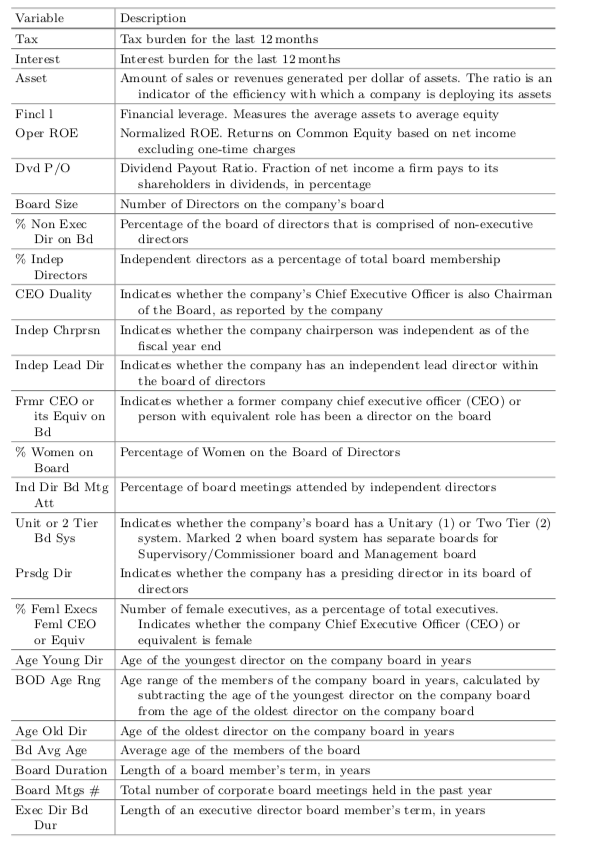
\includegraphics[scale=0.65]{images/var_desc.png}
\end{figure}
\fi

\begin{table}[h!]
\scalebox{0.8}{
\begin{tabular}{ |p{5cm}|p{12cm}| }
 \hline
 {\bf Variable} & {\bf Description}  \\
 \hline
Tax &Tax burden for the last 12 months \\
\rowcolor{gray}Interest&Interest burden for the last 12 months \\
Asset&Amount of sales or revenues generated per dollar of assets. The ratio is an indicator of the efficiency with which a company is deploying its assets \\
\rowcolor{gray}Fincl&Financial leverage. Measures the average assets to average equity \\
Oper ROE&Normalized ROE. Returns on Common Equity based on net income excluding one-time charges \\
\rowcolor{gray}Dvd P/O&Dividend Payout Ratio. Fraction of net income a firm pays to its shareholders in dividends, in percentage \\
Board Size&Number of Directors on the company?s board \\
\rowcolor{gray}\% Non Exec Dir on Bd &Percentage of the board of directors that is comprised of non-executive directors \\
\% Indep Directors &Independent directors as a percentage of total board membership \\
\rowcolor{gray}CEO Duality &Indicates whether the company?s Chief Executive Officer is also Chairman of the Board, as reported by the company \\
Indep Chrprsn&Indicates whether the company chairperson was independent as of the fiscal year end \\
\rowcolor{gray}Indep Lead Dir&Indicates whether the company has an independent lead director within the board of directors \\
Frmr CEO or its Equiv on Bd&Indicates whether a former company chief executive officer (CEO) or person with equivalent role has been a director on the board \\
\rowcolor{gray}\% Women on Board&Percentage of Women on the Board of Directors \\
\hline
\end{tabular}}
\end{table}



\begin{table}[!htb]
\scalebox{0.8}{
\begin{tabular}{ |p{5cm}|p{12cm}| }
 \hline
 {\bf Variable} & {\bf Description}  \\
 \hline
 Ind Dir Db Mtg Att&Percentage of board meetings attended by independent directors \\
\rowcolor{gray}Unit or 2 Tier Bd sys&Indicates whether the company?s board has a Unitary (1) or Two Tier (2) system. Marked 2 when board system has separate boards for Supervisory/Commissioner board and Management board \\
\rowcolor{gray}Prsdg Dir&Indicates whether the company has a presiding director in its board of directors \\
\% Feml Execs Feml CEO or Equiv&Number of female executives, as a percentage of total executives. Indicates whether the company Chief Executive Officer (CEO) or equivalent is female \\
\rowcolor{gray}Age Young Dir &Age of the youngest director on the company board in years \\
BOD Age Rng &Age range of the members of the company board in years, calculated by subtracting the age of the youngest director on the company board from the age of the oldest director on the company board \\
\rowcolor{gray}Age Old Dir&Age of the oldest director on the company board in years Average age of the members of the board \\
Bd Avg Age&Average age of the memebers of the board\\
\rowcolor{gray}Board Duration &Length of a board member?s term, in years \\
Board Mtgs \# &Total number of corporate board meetings held in the past year \\
\rowcolor{gray}Exec Dir Bd Dur &Length of an executive director board member?s term, in years \\
  \hline
\end{tabular}}
\end{table}
\vspace*{4in}


%   MSc Business Analytics Dissertation
%
%   Title:     Aaa Bbbbbbb Cccccccccc
%   Author(s): Xxxxxx Xxxxxxxxx and Yyy Yyyyyyyyy
%
%   Appendix 2: program code
%
%   Change Control:
%   When     Who   Ver  What
%   -------  ----  ---  --------------------------------------------------------------
%   11Feb11  AB    0.1  Begun 
%

\chapter{Program code}\label{C.Appendix2}

Insert snippets of important code here \\
Point to github where code can be found\\\\ 
\url{https://github.com/ReidConor/dissertation}
% and so on

%%   Endnotes (if needed)

%%   Glossary of terms
%%   \include this as it may be big enough to justify its own ``chapter''
\cleardoublepage
\addcontentsline{toc}{chapter}{Glossary}
%   MSc Business Analytics Dissertation
%
%   Title:     Aaa Bbbbbbb Cccccccccc
%   Author(s): Xxxxxx Xxxxxxxxx and Yyy Yyyyyyyyy
%
%   Glossary
%
%   Change Control:
%   When     Who   Ver  What
%   -------  ----  ---  --------------------------------------------------------------
%   11Feb11  AB    0.1  Begun 
%

\chapter*{Glossary}\label{C.Glossary}

Entries are listed in alphabetical order.  



%%   Bibliography (References)
% For this, use BibTeX (invariably comes with your LaTeX installation).  BibTeX separates the form of a
% reference from its content, just as LaTeX does for a document.  You put the content in a .bib file
% called a BibTeX database, and tell BibTeX what style to overlay on it.
\cleardoublepage
\addcontentsline{toc}{chapter}{Bibliography}
\bibliographystyle{mscBA} % the BibTeX style file to use (omit the .bst suffix)
\bibliography{thesis}     % the BibTeX database file to use (omit the .bib suffix)
%
%% In the above, mscBA.bst is a BibTeX style file I developed based on the fairly standard chicago.bst.
%%
%% Below are sample journal and book entries from a .bib file.  Ensure that the key e.g., Chomsky:1965 you use
%% in your .bib file entry is the same as you use in the \cite{Chomsky:1965} command in your LaTeX file.
%%
%% @String{MIT = {{MIT Press}}}
%% @String{MIT:adr = {{Cambridge, Massachusetts}}}
%%
%% @Article{MetropEtAl:1953,
%%  AUTHOR =       {Metropolis, N. and A.W. Rosenbluth and M.N. Rosenbluth and A.H. Teller and E. Teller},
%%  YEAR =         {1953},
%%  TITLE =        {Equations of {S}tate Calculations by Fast Computing Machines},
%%  JOURNAL =      {Journal of Chemical Physics},
%%  VOLUME =       {21},
%%  NUMBER =       {6},
%%  PAGES =        {1087--1092}
%% }
%%
%% @Book{Chomsky:1965,
%%   Author =       {N. Chomsky},
%%   title =        {Aspects of the theory of syntax},
%%   PUBLISHER =    MIT,
%%   ADDRESS =      MIT:adr,
%%   YEAR =         1965
%% }
%%
%% Some other points (see the sample bibfile entries above for illustration):
%% - Case is unimportant for a field name: DATE, daTe and date all mean the same.
%% - You separate multiple authors by 'and', not using commas etc.
%% - Some punctuation marks in the key are OK, e.g. the colon ':' as in MetropEtAl:1953
%% - BibTeX has its own internal rules on when to change the case of capitalised text (e.g. in journal article titles).
%%   You can override this by putting braces {} around text you want unchanged (e.g. the S in the article title above.
%% - You can define strings which will be expanded in the references, e.g., MIT and MIT:adr in the book above
%%   Don't put braces or quotes around these: if you do, they will not be expanded (will remain as MIT:adr, say)
%% - In your actual text, you can cite in two ways (note the position of parentheses):
%%   \citep{MetropEtAl:1953} for citation in parentheses, e.g.,
%%     "In \citep{MetropEtAl:1953} it is shown that ..." appears as "In (Metropolis et al, 1953) it is shown that ..."
%%   \citet{MetropEtAl:1953} for citation in text, e.g., where the authors are the subject of the sentence:
%%     "\citet{MetropEtAl:1953} show that ..." appears as "Metropolis et al (1953) show that ..."
%% - With either \citep or \citet you can use optional arguments such as
%%     "\citep[e.g.,][pp.~12--20]{MetropEtAl:1953}" appears as "(e.g., Metropolis et al, 1953, pp.~12--20)"

%%   List of contributors -- anyone else you feel should be credited

%%   Notation Index / List of Symbols
%%   \include this as it may be big enough to justify its own ``chapter''
\cleardoublepage
\addcontentsline{toc}{chapter}{List of Notation}
%   MSc Business Analytics Dissertation
%
%   Title:     Aaa Bbbbbbb Cccccccccc
%   Author(s): Xxxxxx Xxxxxxxxx and Yyy Yyyyyyyyy
%
%   List of Notation
%
%   Change Control:
%   When     Who   Ver  What
%   -------  ----  ---  --------------------------------------------------------------
%   11Feb11  AB    0.1  Begun 
%

\chapter*{List of Notation}\label{C.Notation}

Entries are listed in the order of appearance.  The ``Ref'' is the number of the section, 
definition, etc., in which the notation is explained.

\vspace{0.5cm}

{\renewcommand{\arraystretch}{0.9}

\begin{tabular}{llr}
\tb{Symbol}  & \tb{Description} & \tb{Ref}   \\\hline
$\FF_q $  & Finite field of $q$ elements & \ref{Th.FF.fte.field}  \\
\end{tabular}


}



%%   Index
\cleardoublepage
\addcontentsline{toc}{chapter}{Index}
\printindex

\end{document}
